\documentclass[sigconf,review]{acmart}
\usepackage{amsmath,booktabs,graphicx,multirow}
\emergencystretch=2em
\setcopyright{none}
\acmConference[KDD '27 D\&B]{ACM SIGKDD Conference on Knowledge Discovery and Data Mining}{2027}{San Jose, CA, USA}
\acmYear{2027}
\acmDOI{}
\acmISBN{}
\newcommand{\repourl}{https://github.com/rain788/idcon-benchmark}
\newcommand{\doiurl}{\href{https://doi.org/10.5281/zenodo.24576233}{10.5281/zenodo.24576233}}
\newcommand{\hardTasks}{504}
\newcommand{\hardAncestors}{72}
\newcommand{\hardComplete}{504}
\newcommand{\hardUnassessed}{0}
\newcommand{\hardFirstWrongPct}{31.2}
\newcommand{\hardFirstWrongAnsweredPct}{33.5}
\newcommand{\hardUnknownSharePct}{31.9}
\newcommand{\hardFirstWrongOnUnknown}{315}
\newcommand{\hardFirstWrong}{315}
\newcommand{\hardFirstAnswered}{941}
\newcommand{\hardFirstAssessed}{1008}
\newcommand{\hardBest}{LAD}
\newcommand{\hardBestUnsolvedPct}{28.1}
\newcommand{\hardBestPar}{1,635}
\newcommand{\hardSecond}{Glasgow}
\newcommand{\hardSecondPar}{2,113}
\newcommand{\hardMost}{LAD}
\newcommand{\hardMostCorrect}{725}
\newcommand{\hardVBSUnsolved}{186}
\newcommand{\hardVBSUnsolvedPct}{18.5}
\newcommand{\hardVBSAllUnsolved}{174}
\newcommand{\hardVBSAllUnsolvedPct}{17.3}
\newcommand{\hardNegVone}{301}
\newcommand{\hardNegVoneCorroborated}{187}
\newcommand{\hardNegRone}{305}
\newcommand{\hardNegRoneCorroborated}{285}
\newcommand{\hardCorroboratedTasks}{487}
\newcommand{\hardPriorScenario}{339/504}
\newcommand{\hardPriorMeta}{368/504}
\newcommand{\hardPriorLearned}{419/504}
\newcommand{\hardPriorLearnedPct}{83.1}
\newcommand{\hardSymExplained}{0}
\newcommand{\hardSymUnknown}{161}
\newcommand{\hardLADCorrect}{725}
\newcommand{\hardLADAssessed}{1008}
\newcommand{\hardLADPar}{1,635}
\newcommand{\hardLADWrong}{0}
\newcommand{\hardLADParTen}{1,635}
\newcommand{\hardGlasgowCorrect}{562}
\newcommand{\hardGlasgowAssessed}{1008}
\newcommand{\hardGlasgowPar}{2,113}
\newcommand{\hardGlasgowWrong}{0}
\newcommand{\hardGlasgowParTen}{2,113}
\newcommand{\hardGlasgowstagedCorrect}{651}
\newcommand{\hardGlasgowstagedAssessed}{1008}
\newcommand{\hardGlasgowstagedPar}{1,740}
\newcommand{\hardGlasgowstagedWrong}{0}
\newcommand{\hardGlasgowstagedParTen}{1,740}
\newcommand{\hardCPSATCorrect}{321}
\newcommand{\hardCPSATAssessed}{1008}
\newcommand{\hardCPSATPar}{2,998}
\newcommand{\hardCPSATWrong}{0}
\newcommand{\hardCPSATParTen}{2,998}
\newcommand{\hardTradCPCorrect}{214}
\newcommand{\hardTradCPAssessed}{1008}
\newcommand{\hardTradCPPar}{3,347}
\newcommand{\hardTradCPWrong}{0}
\newcommand{\hardTradCPParTen}{3,347}
\newcommand{\hardEnumGlasgowCorrect}{88}
\newcommand{\hardEnumGlasgowAssessed}{1008}
\newcommand{\hardEnumGlasgowPar}{3,688}
\newcommand{\hardEnumGlasgowWrong}{0}
\newcommand{\hardEnumGlasgowParTen}{3,688}
\newcommand{\hardEnumVFTwoCorrect}{14}
\newcommand{\hardEnumVFTwoAssessed}{1008}
\newcommand{\hardEnumVFTwoPar}{3,951}
\newcommand{\hardEnumVFTwoWrong}{0}
\newcommand{\hardEnumVFTwoParTen}{3,951}
\newcommand{\hardASPcautiousCorrect}{15}
\newcommand{\hardASPcautiousAssessed}{1008}
\newcommand{\hardASPcautiousPar}{3,968}
\newcommand{\hardASPcautiousWrong}{0}
\newcommand{\hardASPcautiousParTen}{3,968}
\newcommand{\hardSATCorrect}{240}
\newcommand{\hardSATAssessed}{1008}
\newcommand{\hardSATPar}{3,378}
\newcommand{\hardSATWrong}{0}
\newcommand{\hardSATParTen}{3,378}
\newcommand{\hardFirstmatchCorrect}{626}
\newcommand{\hardFirstmatchAssessed}{1008}
\newcommand{\hardFirstmatchPar}{1,901}
\newcommand{\hardFirstmatchWrong}{315}
\newcommand{\hardFirstmatchParTen}{6,901}
\newcommand{\hardLADTenS}{460}
\newcommand{\hardLADTwoSRepZero}{364}
\newcommand{\hardGlasgowstagedTenS}{400}
\newcommand{\hardGlasgowstagedTwoSRepZero}{326}
\newcommand{\hardCPSATTenS}{231}
\newcommand{\hardCPSATTwoSRepZero}{159}
\newcommand{\hardEnumGlasgowTenS}{44}
\newcommand{\hardEnumGlasgowTwoSRepZero}{44}
\newcommand{\hardRepZeroN}{504}
\newcommand{\hprdTasks}{200}
\newcommand{\hprdAncestors}{100}
\newcommand{\hprdComplete}{200}
\newcommand{\hprdUnassessed}{0}
\newcommand{\hprdFirstWrongPct}{42.5}
\newcommand{\hprdFirstWrongAnsweredPct}{42.5}
\newcommand{\hprdUnknownSharePct}{42.5}
\newcommand{\hprdFirstWrongOnUnknown}{170}
\newcommand{\hprdFirstWrong}{170}
\newcommand{\hprdFirstAnswered}{400}
\newcommand{\hprdFirstAssessed}{400}
\newcommand{\hprdBest}{SAT}
\newcommand{\hprdBestUnsolvedPct}{0.0}
\newcommand{\hprdBestPar}{374}
\newcommand{\hprdSecond}{CP-SAT}
\newcommand{\hprdSecondPar}{455}
\newcommand{\hprdMost}{SAT}
\newcommand{\hprdMostCorrect}{400}
\newcommand{\hprdVBSUnsolved}{0}
\newcommand{\hprdVBSUnsolvedPct}{0.0}
\newcommand{\hprdVBSAllUnsolved}{0}
\newcommand{\hprdVBSAllUnsolvedPct}{0.0}
\newcommand{\hprdNegVone}{115}
\newcommand{\hprdNegVoneCorroborated}{115}
\newcommand{\hprdNegRone}{115}
\newcommand{\hprdNegRoneCorroborated}{115}
\newcommand{\hprdCorroboratedTasks}{200}
\newcommand{\hprdPriorScenario}{183/200}
\newcommand{\hprdPriorMeta}{183/200}
\newcommand{\hprdPriorLearned}{181/200}
\newcommand{\hprdPriorLearnedPct}{90.5}
\newcommand{\hprdSymExplained}{0}
\newcommand{\hprdSymUnknown}{85}
\newcommand{\hprdLADCorrect}{389}
\newcommand{\hprdLADAssessed}{400}
\newcommand{\hprdLADPar}{1,036}
\newcommand{\hprdLADWrong}{0}
\newcommand{\hprdLADParTen}{1,036}
\newcommand{\hprdGlasgowCorrect}{0}
\newcommand{\hprdGlasgowAssessed}{400}
\newcommand{\hprdGlasgowPar}{4,000}
\newcommand{\hprdGlasgowWrong}{0}
\newcommand{\hprdGlasgowParTen}{4,000}
\newcommand{\hprdGlasgowstagedCorrect}{304}
\newcommand{\hprdGlasgowstagedAssessed}{400}
\newcommand{\hprdGlasgowstagedPar}{1,361}
\newcommand{\hprdGlasgowstagedWrong}{0}
\newcommand{\hprdGlasgowstagedParTen}{1,361}
\newcommand{\hprdCPSATCorrect}{384}
\newcommand{\hprdCPSATAssessed}{400}
\newcommand{\hprdCPSATPar}{455}
\newcommand{\hprdCPSATWrong}{0}
\newcommand{\hprdCPSATParTen}{455}
\newcommand{\hprdTradCPCorrect}{279}
\newcommand{\hprdTradCPAssessed}{400}
\newcommand{\hprdTradCPPar}{1,858}
\newcommand{\hprdTradCPWrong}{0}
\newcommand{\hprdTradCPParTen}{1,858}
\newcommand{\hprdEnumGlasgowCorrect}{235}
\newcommand{\hprdEnumGlasgowAssessed}{400}
\newcommand{\hprdEnumGlasgowPar}{2,638}
\newcommand{\hprdEnumGlasgowWrong}{0}
\newcommand{\hprdEnumGlasgowParTen}{2,638}
\newcommand{\hprdEnumVFTwoCorrect}{127}
\newcommand{\hprdEnumVFTwoAssessed}{400}
\newcommand{\hprdEnumVFTwoPar}{2,937}
\newcommand{\hprdEnumVFTwoWrong}{0}
\newcommand{\hprdEnumVFTwoParTen}{2,937}
\newcommand{\hprdASPcautiousCorrect}{400}
\newcommand{\hprdASPcautiousAssessed}{400}
\newcommand{\hprdASPcautiousPar}{748}
\newcommand{\hprdASPcautiousWrong}{0}
\newcommand{\hprdASPcautiousParTen}{748}
\newcommand{\hprdSATCorrect}{400}
\newcommand{\hprdSATAssessed}{400}
\newcommand{\hprdSATPar}{374}
\newcommand{\hprdSATWrong}{0}
\newcommand{\hprdSATParTen}{374}
\newcommand{\hprdFirstmatchCorrect}{230}
\newcommand{\hprdFirstmatchAssessed}{400}
\newcommand{\hprdFirstmatchPar}{2,027}
\newcommand{\hprdFirstmatchWrong}{170}
\newcommand{\hprdFirstmatchParTen}{8,827}
\newcommand{\hprdLADTenS}{200}
\newcommand{\hprdLADTwoSRepZero}{195}
\newcommand{\hprdGlasgowTenS}{184}
\newcommand{\hprdGlasgowTwoSRepZero}{0}
\newcommand{\hprdGlasgowstagedTenS}{194}
\newcommand{\hprdGlasgowstagedTwoSRepZero}{153}
\newcommand{\hprdCPSATTenS}{196}
\newcommand{\hprdCPSATTwoSRepZero}{192}
\newcommand{\hprdEnumGlasgowTenS}{198}
\newcommand{\hprdEnumGlasgowTwoSRepZero}{118}
\newcommand{\hprdRepZeroN}{200}
\newcommand{\hprdxTasks}{192}
\newcommand{\hprdxAncestors}{96}
\newcommand{\hprdxComplete}{192}
\newcommand{\hprdxUnassessed}{0}
\newcommand{\hprdxFirstWrongPct}{41.7}
\newcommand{\hprdxFirstWrongAnsweredPct}{41.7}
\newcommand{\hprdxUnknownSharePct}{41.7}
\newcommand{\hprdxFirstWrongOnUnknown}{160}
\newcommand{\hprdxFirstWrong}{160}
\newcommand{\hprdxFirstAnswered}{384}
\newcommand{\hprdxFirstAssessed}{384}
\newcommand{\hprdxBest}{SAT}
\newcommand{\hprdxBestUnsolvedPct}{0.0}
\newcommand{\hprdxBestPar}{380}
\newcommand{\hprdxSecond}{CP-SAT}
\newcommand{\hprdxSecondPar}{830}
\newcommand{\hprdxMost}{SAT}
\newcommand{\hprdxMostCorrect}{384}
\newcommand{\hprdxVBSUnsolved}{3}
\newcommand{\hprdxVBSUnsolvedPct}{0.8}
\newcommand{\hprdxVBSAllUnsolved}{0}
\newcommand{\hprdxVBSAllUnsolvedPct}{0.0}
\newcommand{\hprdxNegVone}{112}
\newcommand{\hprdxNegVoneCorroborated}{111}
\newcommand{\hprdxNegRone}{112}
\newcommand{\hprdxNegRoneCorroborated}{111}
\newcommand{\hprdxCorroboratedTasks}{191}
\newcommand{\hprdxPriorScenario}{170/192}
\newcommand{\hprdxPriorMeta}{164/192}
\newcommand{\hprdxPriorLearned}{166/192}
\newcommand{\hprdxPriorLearnedPct}{86.5}
\newcommand{\hprdxSymExplained}{1}
\newcommand{\hprdxSymUnknown}{80}
\newcommand{\hprdxLADCorrect}{199}
\newcommand{\hprdxLADAssessed}{384}
\newcommand{\hprdxLADPar}{2,513}
\newcommand{\hprdxLADWrong}{0}
\newcommand{\hprdxLADParTen}{2,513}
\newcommand{\hprdxGlasgowCorrect}{1}
\newcommand{\hprdxGlasgowAssessed}{384}
\newcommand{\hprdxGlasgowPar}{3,995}
\newcommand{\hprdxGlasgowWrong}{0}
\newcommand{\hprdxGlasgowParTen}{3,995}
\newcommand{\hprdxGlasgowstagedCorrect}{265}
\newcommand{\hprdxGlasgowstagedAssessed}{384}
\newcommand{\hprdxGlasgowstagedPar}{1,734}
\newcommand{\hprdxGlasgowstagedWrong}{0}
\newcommand{\hprdxGlasgowstagedParTen}{1,734}
\newcommand{\hprdxCPSATCorrect}{360}
\newcommand{\hprdxCPSATAssessed}{384}
\newcommand{\hprdxCPSATPar}{830}
\newcommand{\hprdxCPSATWrong}{0}
\newcommand{\hprdxCPSATParTen}{830}
\newcommand{\hprdxTradCPCorrect}{191}
\newcommand{\hprdxTradCPAssessed}{384}
\newcommand{\hprdxTradCPPar}{2,603}
\newcommand{\hprdxTradCPWrong}{0}
\newcommand{\hprdxTradCPParTen}{2,603}
\newcommand{\hprdxEnumGlasgowCorrect}{65}
\newcommand{\hprdxEnumGlasgowAssessed}{384}
\newcommand{\hprdxEnumGlasgowPar}{3,568}
\newcommand{\hprdxEnumGlasgowWrong}{0}
\newcommand{\hprdxEnumGlasgowParTen}{3,568}
\newcommand{\hprdxEnumVFTwoCorrect}{74}
\newcommand{\hprdxEnumVFTwoAssessed}{384}
\newcommand{\hprdxEnumVFTwoPar}{3,354}
\newcommand{\hprdxEnumVFTwoWrong}{0}
\newcommand{\hprdxEnumVFTwoParTen}{3,354}
\newcommand{\hprdxASPcautiousCorrect}{365}
\newcommand{\hprdxASPcautiousAssessed}{384}
\newcommand{\hprdxASPcautiousPar}{1,230}
\newcommand{\hprdxASPcautiousWrong}{0}
\newcommand{\hprdxASPcautiousParTen}{1,230}
\newcommand{\hprdxSATCorrect}{384}
\newcommand{\hprdxSATAssessed}{384}
\newcommand{\hprdxSATPar}{380}
\newcommand{\hprdxSATWrong}{0}
\newcommand{\hprdxSATParTen}{380}
\newcommand{\hprdxFirstmatchCorrect}{224}
\newcommand{\hprdxFirstmatchAssessed}{384}
\newcommand{\hprdxFirstmatchPar}{2,242}
\newcommand{\hprdxFirstmatchWrong}{160}
\newcommand{\hprdxFirstmatchParTen}{8,909}
\newcommand{\hprdCountFullQueries}{100}
\newcommand{\hprdCountFullMulti}{93}
\newcommand{\hprdCountFullThousand}{2}
\newcommand{\hprdCountFullUnique}{7}
\newcommand{\hprdCountFullTimeouts}{0}
\newcommand{\hprdCountSpaceQueries}{100}
\newcommand{\hprdCountSpaceMulti}{97}
\newcommand{\hprdCountSpaceThousand}{28}
\newcommand{\hprdCountSpaceUnique}{3}
\newcommand{\hprdCountSpaceTimeouts}{1}
\newcommand{\hprdxCountFullQueries}{96}
\newcommand{\hprdxCountFullMulti}{90}
\newcommand{\hprdxCountFullThousand}{18}
\newcommand{\hprdxCountFullUnique}{6}
\newcommand{\hprdxCountFullTimeouts}{0}
\newcommand{\hprdxCountSpaceQueries}{96}
\newcommand{\hprdxCountSpaceMulti}{95}
\newcommand{\hprdxCountSpaceThousand}{47}
\newcommand{\hprdxCountSpaceUnique}{1}
\newcommand{\hprdxCountSpaceTimeouts}{4}
\newcommand{\ovhWriteHostGraph}{20}
\newcommand{\ovhLadOneRole}{759}
\newcommand{\ovhGlasgowOneRole}{1,003}
\newcommand{\ovhGlasgowStagedOneRole}{170}
\newcommand{\ovhGraphData}{32}
\newcommand{\totalTasks}{896}
\newcommand{\totalAncestors}{268}
\newcommand{\hprdFirstWrongSpecTrue}{168}
\newcommand{\hprdFirstWrongSpecTrueVio}{158}
\newcommand{\hprdFirstWrongSpecTrueSat}{10}
\newcommand{\hprdFirstWrongSpecWrong}{2}
\newcommand{\hardRepeatAgreePct}{98.6}
\newcommand{\hprdRepeatAgreePct}{97.9}
\newcommand{\hprdxRepeatAgreePct}{91.5}
\newcommand{\witnessTotal}{12,621}
\newcommand{\strataSentence}{on IdCon-Hard the best method is LAD in 2k plain (0.75, n.s.), 4k plain (1.00) and 8k constr. (0.75, n.s.); Glasgow in 8k plain (0.99); CP-SAT in 2k constr. (0.63, n.s.) and 4k constr. (1.00), and on IdCon-HPRD-X the best method is SAT$^\ddagger$ in 8d (0.99), 8s (1.00), 16d (1.00), 16s (1.00), 24d (1.00), 24s (1.00), 32d (1.00) and 32s (1.00)}
\newcommand{\vbsUnsolvedSentence}{105 are \Sat{}, 32 are \Vio{}, 39 are \Unk{} and 10 are \Emp{}}
\newcommand{\hardLADSatCorrect}{165}
\newcommand{\hardGlasgowSatCorrect}{104}
\newcommand{\hardGlasgowstagedSatCorrect}{125}
\newcommand{\hardCPSATSatCorrect}{145}
\newcommand{\hardTradCPSatCorrect}{59}
\newcommand{\hardEnumGlasgowSatCorrect}{24}
\newcommand{\hardEnumVFTwoSatCorrect}{0}
\newcommand{\hardASPcautiousSatCorrect}{6}
\newcommand{\hardSATSatCorrect}{99}
\newcommand{\hardFirstmatchSatCorrect}{306}
\newcommand{\hardLADUnkCorrect}{261}
\newcommand{\hardGlasgowUnkCorrect}{237}
\newcommand{\hardGlasgowstagedUnkCorrect}{262}
\newcommand{\hardCPSATUnkCorrect}{37}
\newcommand{\hardTradCPUnkCorrect}{68}
\newcommand{\hardEnumGlasgowUnkCorrect}{26}
\newcommand{\hardEnumVFTwoUnkCorrect}{6}
\newcommand{\hardASPcautiousUnkCorrect}{6}
\newcommand{\hardSATUnkCorrect}{45}
\newcommand{\hardFirstmatchUnkCorrect}{6}
\newcommand{\hardLADVioCorrect}{221}
\newcommand{\hardGlasgowVioCorrect}{169}
\newcommand{\hardGlasgowstagedVioCorrect}{197}
\newcommand{\hardCPSATVioCorrect}{80}
\newcommand{\hardTradCPVioCorrect}{49}
\newcommand{\hardEnumGlasgowVioCorrect}{12}
\newcommand{\hardEnumVFTwoVioCorrect}{0}
\newcommand{\hardASPcautiousVioCorrect}{3}
\newcommand{\hardSATVioCorrect}{62}
\newcommand{\hardFirstmatchVioCorrect}{235}
\newcommand{\hardLADEmpCorrect}{78}
\newcommand{\hardGlasgowEmpCorrect}{52}
\newcommand{\hardGlasgowstagedEmpCorrect}{67}
\newcommand{\hardCPSATEmpCorrect}{59}
\newcommand{\hardTradCPEmpCorrect}{38}
\newcommand{\hardEnumGlasgowEmpCorrect}{26}
\newcommand{\hardEnumVFTwoEmpCorrect}{8}
\newcommand{\hardASPcautiousEmpCorrect}{0}
\newcommand{\hardSATEmpCorrect}{34}
\newcommand{\hardFirstmatchEmpCorrect}{79}
\newcommand{\refEgSentence}{The 3 IdCon-Hard tasks whose v1 references had been settled by a solver that is no longer part of the benchmark were re-settled without it: 3 with the same label.}
\newcommand{\refRankSentence}{is unchanged on every suite}

\newcommand{\totalTasksRtwo}{1,160}
\newcommand{\totalAncestorsRtwo}{376}
\newcommand{\hardxTasks}{72}
\newcommand{\hardxAncestors}{12}
\newcommand{\hardxComplete}{68}
\newcommand{\hardxUnassessed}{4}
\newcommand{\hardxLabels}{21/9/30/8}
\newcommand{\hardxPriorScenario}{45/68}
\newcommand{\hardxPriorMeta}{38/68}
\newcommand{\hardxPriorLearned}{52/68}
\newcommand{\hardxVBSUnsolvedTwo}{49}
\newcommand{\hardxVBSUnsolvedTen}{23}
\newcommand{\hardxVBSUnsolvedSixty}{3}
\newcommand{\hardxEnumGlasgowTwo}{1}
\newcommand{\hardxEnumGlasgowTen}{4}
\newcommand{\hardxEnumGlasgowSixty}{4}
\newcommand{\hardxFirstmatchTwo}{1}
\newcommand{\hardxFirstmatchTen}{35}
\newcommand{\hardxFirstmatchSixty}{35}
\newcommand{\hardxGlasgowTwo}{1}
\newcommand{\hardxGlasgowTen}{29}
\newcommand{\hardxGlasgowSixty}{29}
\newcommand{\hardxGlasgowstagedTwo}{15}
\newcommand{\hardxGlasgowstagedTen}{33}
\newcommand{\hardxGlasgowstagedSixty}{46}
\newcommand{\hardxLADTwo}{1}
\newcommand{\hardxLADTen}{30}
\newcommand{\hardxLADSixty}{64}
\newcommand{\hardxSATTwo}{2}
\newcommand{\hardxSATTen}{2}
\newcommand{\hardxSATSixty}{40}
\newcommand{\hardxCPSATTwo}{5}
\newcommand{\hardxCPSATTen}{11}
\newcommand{\hardxCPSATSixty}{11}
\newcommand{\hardxBestSingleTwo}{Glasgow-staged}
\newcommand{\hardxBestSingleTwoN}{15}
\newcommand{\hardxBestSingleTen}{Glasgow-staged}
\newcommand{\hardxBestSingleTenN}{33}
\newcommand{\hardxBestSingleSixty}{LAD}
\newcommand{\hardxBestSingleSixtyN}{64}
\newcommand{\hardxBest}{Glasgow-staged}
\newcommand{\hardxBestPar}{3,346}
\newcommand{\hardxCertWrong}{0}
\newcommand{\hardxFirstWrong}{0}
\newcommand{\hardxFirstAnswered}{1}
\newcommand{\citeTasks}{192}
\newcommand{\citeAncestors}{96}
\newcommand{\citeComplete}{192}
\newcommand{\citeUnassessed}{0}
\newcommand{\citeLabels}{14/52/126/0}
\newcommand{\citePriorScenario}{134/192}
\newcommand{\citePriorMeta}{162/192}
\newcommand{\citePriorLearned}{162/192}
\newcommand{\citeVBSUnsolvedTwo}{55}
\newcommand{\citeVBSUnsolvedTen}{0}
\newcommand{\citeVBSUnsolvedSixty}{0}
\newcommand{\citeASPcautiousTwo}{111}
\newcommand{\citeASPcautiousTen}{192}
\newcommand{\citeASPcautiousSixty}{192}
\newcommand{\citeEnumGlasgowTwo}{53}
\newcommand{\citeEnumGlasgowTen}{53}
\newcommand{\citeEnumGlasgowSixty}{53}
\newcommand{\citeEnumVFTwoTwo}{38}
\newcommand{\citeEnumVFTwoTen}{38}
\newcommand{\citeEnumVFTwoSixty}{38}
\newcommand{\citeFirstmatchTwo}{57}
\newcommand{\citeFirstmatchTen}{57}
\newcommand{\citeFirstmatchSixty}{57}
\newcommand{\citeGlasgowTwo}{47}
\newcommand{\citeGlasgowTen}{47}
\newcommand{\citeGlasgowSixty}{47}
\newcommand{\citeGlasgowstagedTwo}{63}
\newcommand{\citeGlasgowstagedTen}{107}
\newcommand{\citeGlasgowstagedSixty}{107}
\newcommand{\citeLADTwo}{96}
\newcommand{\citeLADTen}{191}
\newcommand{\citeLADSixty}{191}
\newcommand{\citeSATTwo}{133}
\newcommand{\citeSATTen}{192}
\newcommand{\citeSATSixty}{192}
\newcommand{\citeTradCPTwo}{95}
\newcommand{\citeTradCPTen}{95}
\newcommand{\citeTradCPSixty}{95}
\newcommand{\citeCPSATTwo}{62}
\newcommand{\citeCPSATTen}{88}
\newcommand{\citeCPSATSixty}{88}
\newcommand{\citeBestSingleTwo}{SAT}
\newcommand{\citeBestSingleTwoN}{133}
\newcommand{\citeBestSingleTen}{ASP-cautious}
\newcommand{\citeBestSingleTenN}{192}
\newcommand{\citeBestSingleSixty}{ASP-cautious}
\newcommand{\citeBestSingleSixtyN}{192}
\newcommand{\citeBest}{SAT}
\newcommand{\citeBestPar}{1,598}
\newcommand{\citeCertWrong}{0}
\newcommand{\citeFirstWrong}{80}
\newcommand{\citeFirstAnswered}{194}
\newcommand{\hardhTasks}{72}
\newcommand{\witnessTotalRtwo}{17,747}
\newcommand{\hardxNeg}{33}
\newcommand{\hardxNegCorroborated}{4}
\newcommand{\citeNeg}{66}
\newcommand{\citeNegCorroborated}{57}
\newcommand{\hardhCommit}{5da9e1e2b06d}
\newcommand{\citeRuns}{384}
\newcommand{\citeVBSUnsolvedRuns}{110}
\newcommand{\hardLadRepTwo}{364}
\newcommand{\hardLadRepTen}{460}
\newcommand{\hardLadRepSixty}{498}
\newcommand{\hardGSRepTwo}{326}
\newcommand{\hardGSRepTen}{400}
\newcommand{\hardGSRepSixty}{429}
\newcommand{\hardVBSAllUnsolvedTwo}{87}
\newcommand{\hardVBSAllUnsolvedTen}{22}
\newcommand{\hardVBSAllUnsolvedSixty}{4}
\newcommand{\hardVBSROneUnsolvedTwo}{93}
\newcommand{\hardVBSROneUnsolvedTen}{22}
\newcommand{\hardVBSROneUnsolvedSixty}{4}
\newcommand{\hardSixtyRuns}{170}
\newcommand{\hardVBSSixtyLabels}{4 \Sat{}}
\newcommand{\legEgCorrect}{861}
\newcommand{\legEgPar}{874}
\newcommand{\legEgUnans}{147}
\newcommand{\legSvCorrect}{799}
\newcommand{\legSvPar}{1,352}
\newcommand{\legVBSEg}{34}
\newcommand{\legVBSBoth}{29}
\newcommand{\legEgUnsolvedPct}{14.6}
\newcommand{\sensDecided}{113}
\newcommand{\sensDecidedDecoyS}{70}
\newcommand{\sensDecidedPct}{22.4}
\newcommand{\sensRankSentence}{the order of the three fastest sound methods (LAD, Glasgow-staged, Glasgow) is the same on all three subsets}
\newcommand{\idcTasks}{292}
\newcommand{\idcAgree}{279}
\newcommand{\idcDisagree}{0}
\newcommand{\idcUnresolved}{12}
\newcommand{\idcDecided}{280}
\newcommand{\idcSettles}{1}
\newcommand{\idcDrat}{131}
\newcommand{\idcUnconfAgree}{10}
\newcommand{\idcUnconfTasks}{17}
\newcommand{\idcCiteAgree}{192}
\newcommand{\idcCiteTasks}{192}
\newcommand{\idcCiteUnresolved}{0}
\newcommand{\idcHardxSingleAgree}{19}
\newcommand{\idcHardxSingleTasks}{19}
\newcommand{\idcHardxSingleUnresolved}{0}
\newcommand{\idcHardxSampleAgree}{10}
\newcommand{\idcHardxSampleTasks}{12}
\newcommand{\idcHardxSampleUnresolved}{1}
\newcommand{\idcRandAgree}{44}
\newcommand{\idcRandTasks}{48}
\newcommand{\priorWrongAllThree}{35}
\newcommand{\priorWrongLearned}{85}
\newcommand{\calibRuns}{100}
\newcommand{\calibAgree}{95}
\newcommand{\calibRatio}{1.27}
\newcommand{\calibBoth}{77}
\newcommand{\hprdAutoOrbitMulti}{92}
\newcommand{\hprdxAutoOrbitMulti}{89}
\newcommand{\ovhHardLadTotal}{704}
\newcommand{\ovhHardLadSolver}{217}
\newcommand{\ovhHardLadOutside}{230}
\newcommand{\ovhHardLadReported}{130}
\newcommand{\ovhHardGSTotal}{474}
\newcommand{\ovhHardGSSolver}{174}
\newcommand{\ovhHardGSOutside}{165}
\newcommand{\ovhHardGSReported}{97}

\newcommand{\regROne}{33f4077}
\newcommand{\regRTwo}{2d67a5f}
\newcommand{\regAsix}{5680c3d}
\newcommand{\regAseven}{ad99dac}
\newcommand{\vOneOne}{be8c3b6}
\newcommand{\archiveSentence}{releases are tagged, and the accepted version will be archived with a DOI}
\ifdefined\IdConAnon
\renewcommand{\repourl}{https://anonymous.4open.science/r/idcon-benchmark}
\renewcommand{\doiurl}{(withheld for review)}
\renewcommand{\regROne}{(withheld)}
\renewcommand{\regRTwo}{(withheld)}
\renewcommand{\regAsix}{(withheld)}
\renewcommand{\regAseven}{(withheld)}
\renewcommand{\vOneOne}{(withheld)}
\renewcommand{\archiveSentence}{releases are tagged, and the accepted version will be archived with a DOI}
\fi

\newcommand{\Sat}{\textsc{Satisfies}}
\newcommand{\Vio}{\textsc{Violates}}
\newcommand{\Unk}{\textsc{Unknown}}
\newcommand{\Emp}{\textsc{Empty}}
\begin{document}
\title{IdCon: A Benchmark for Identity-Consensus Diagnosis over Ambiguous Graph Embeddings}
\author{Yulin Liu}
\authornote{These authors contributed equally to this work.}
\author{Zhiyu Liu}
\authornotemark[1]
\author{Ru Wang}
\authornote{Corresponding author.}
\email{ru.wang13@bit.edu.cn}
\affiliation{%
  \institution{School of Mechanical Engineering, Beijing Institute of Technology}
  \streetaddress{No. 5 Zhongguancun South Street, Haidian District}
  \city{Beijing}
  \postcode{100081}
  \country{China}
}
\renewcommand{\shortauthors}{Liu et al.}

\begin{abstract}
A requirement expressed as a pattern graph is often checked against an observed graph by finding \emph{one} embedding and reading the observations at the matched entities. When several embeddings are admissible and carry different observations, that answer depends on search order. We formalize \emph{identity-consensus diagnosis}: decide whether every admissible embedding satisfies the checked observations, whether every one violates them, whether the evidence is mixed or missing, or whether no admissible embedding exists. We release IdCon, a benchmark of five scored suites and two held-out splits: synthetic IdCon-Hard (504 tasks, hosts of up to 8,192 entities) and IdCon-Hard-X (\hardxTasks{} tasks on 16,384-entity hosts); IdCon-HPRD and IdCon-HPRD-X (200 and 192 tasks on the HPRD protein network with third-party query graphs); and IdCon-Cite (\citeTasks{} tasks on the Cora and PubMed citation graphs with their real labels). Positive reference states are replayed witnesses; negative states are confirmed by a second engine, and an independent encoding with DRAT-checked proofs, run on \idcTasks{} sampled and new-suite tasks, agrees with \idcAgree{} references and contradicts \idcDisagree{}. Embeddings are rarely unique: \hprdAutoOrbitMulti{} of \hprdCountFullQueries{} third-party HPRD queries have more than one embedding up to query symmetry, so a first-match check is wrong on every task whose embeddings disagree. Across nine exact methods (two-query adapters for LAD2025, Glasgow, CP-SAT and a classical CP solver; enumeration; cautious reasoning with clingo; a SAT encoding with CaDiCaL) no certified answer contradicts a reference and no method dominates: \hardBest{} leads on IdCon-Hard, \hardxBest{} on IdCon-Hard-X, and \hprdBest{} on the HPRD suites and IdCon-Cite. Difficulty depends on the budget and the suite: with 10\,s the methods jointly leave \hardVBSAllUnsolvedTen{} of 504 IdCon-Hard tasks unanswered, whereas on IdCon-Hard-X they leave \hardxVBSUnsolvedTen{} of \hardxComplete{} at 10\,s and the best single method needs 60\,s to answer \hardxBestSingleSixtyN{}. Code, data, references, predictions and the design records fixed before each stage of the study are public.

\end{abstract}

\begin{CCSXML}
<ccs2012><concept><concept_id>10002951.10002952.10002953.10010146</concept_id><concept_desc>Information systems~Graph-based database models</concept_desc><concept_significance>500</concept_significance></concept></ccs2012>
\end{CCSXML}
\ccsdesc[500]{Information systems~Graph-based database models}
\keywords{subgraph matching, certain answers, identity uncertainty, benchmark, graph diagnosis}
\maketitle

\section{Introduction}
Engineering, biological and knowledge graphs are checked against requirement patterns. A pattern graph names \emph{roles} (a pump, a supporting beam, a protein with a given function), and the check asks whether the entities that play those roles in an observed graph carry the expected observations. A natural implementation finds one embedding of the pattern with a subgraph matcher and reads the observations at the matched entities. This is correct only when the embedding is unique, and it often is not: in the third-party HPRD query workload that IdCon uses, \hprdAutoOrbitMulti{} of \hprdCountFullQueries{} queries have more than one embedding even when every query vertex must match its own protein label and embeddings that differ only by a symmetry of the query are counted once (Section~\ref{sec:firstmatch}). When two admissible embeddings disagree, the answer of the first match is an accident of search order.

Figure~\ref{fig:task} gives the smallest instance. One embedding maps a checked role to an entity observed as satisfactory, another to an entity observed as violating. A first-match checker reports \Sat{} or \Vio{}, depending on which embedding it meets first. The defensible answer is \Unk{}: the requirement does not hold for every admissible identity, and neither does its negation. If no embedding exists at all, the requirement cannot be placed in the observed graph, which is a different finding from an observed violation.

We call this question \emph{identity-consensus diagnosis}. It is the certain-answer question of incomplete-information databases \cite{imielinski,libkin2014} instantiated over the finite space of injective pattern embeddings, with a three-level observation order on top. It is easy to state and to get wrong, yet no public benchmark measures whether a system answers it or what exact solvers and off-the-shelf certain-answer tools cost on it.

\paragraph{Contributions.} (1) A task definition with four outcomes and a two-query reduction that turns any exact subgraph engine with unary domain restrictions into a consensus solver (Section~\ref{sec:task}). (2) IdCon: two synthetic suites of increasing size, two suites whose graph, labels and query patterns are third-party, a suite on two real citation graphs with their real labels, and two held-out splits; \totalTasksRtwo{} scored tasks over \totalAncestorsRtwo{} pattern--host ancestors (Section~\ref{sec:bench}). (3) References whose positive states are replayed witnesses and whose negative states are confirmed by a second engine and, on a sample and on the new suites, by an independent encoding with checked DRAT proofs; a scoring rule that keeps unsound methods out of the runtime ranking; and a study run in three stages, each fixed by a released design record before its runs (Section~\ref{sec:protocol}). (4) An evaluation of nine exact methods, all built on third-party solvers, which shows that they are sound but none dominates, how the difficulty depends on the budget and the suite, and how much of the label signal is available without search (Section~\ref{sec:results}).

\begin{figure}[t]
\centering
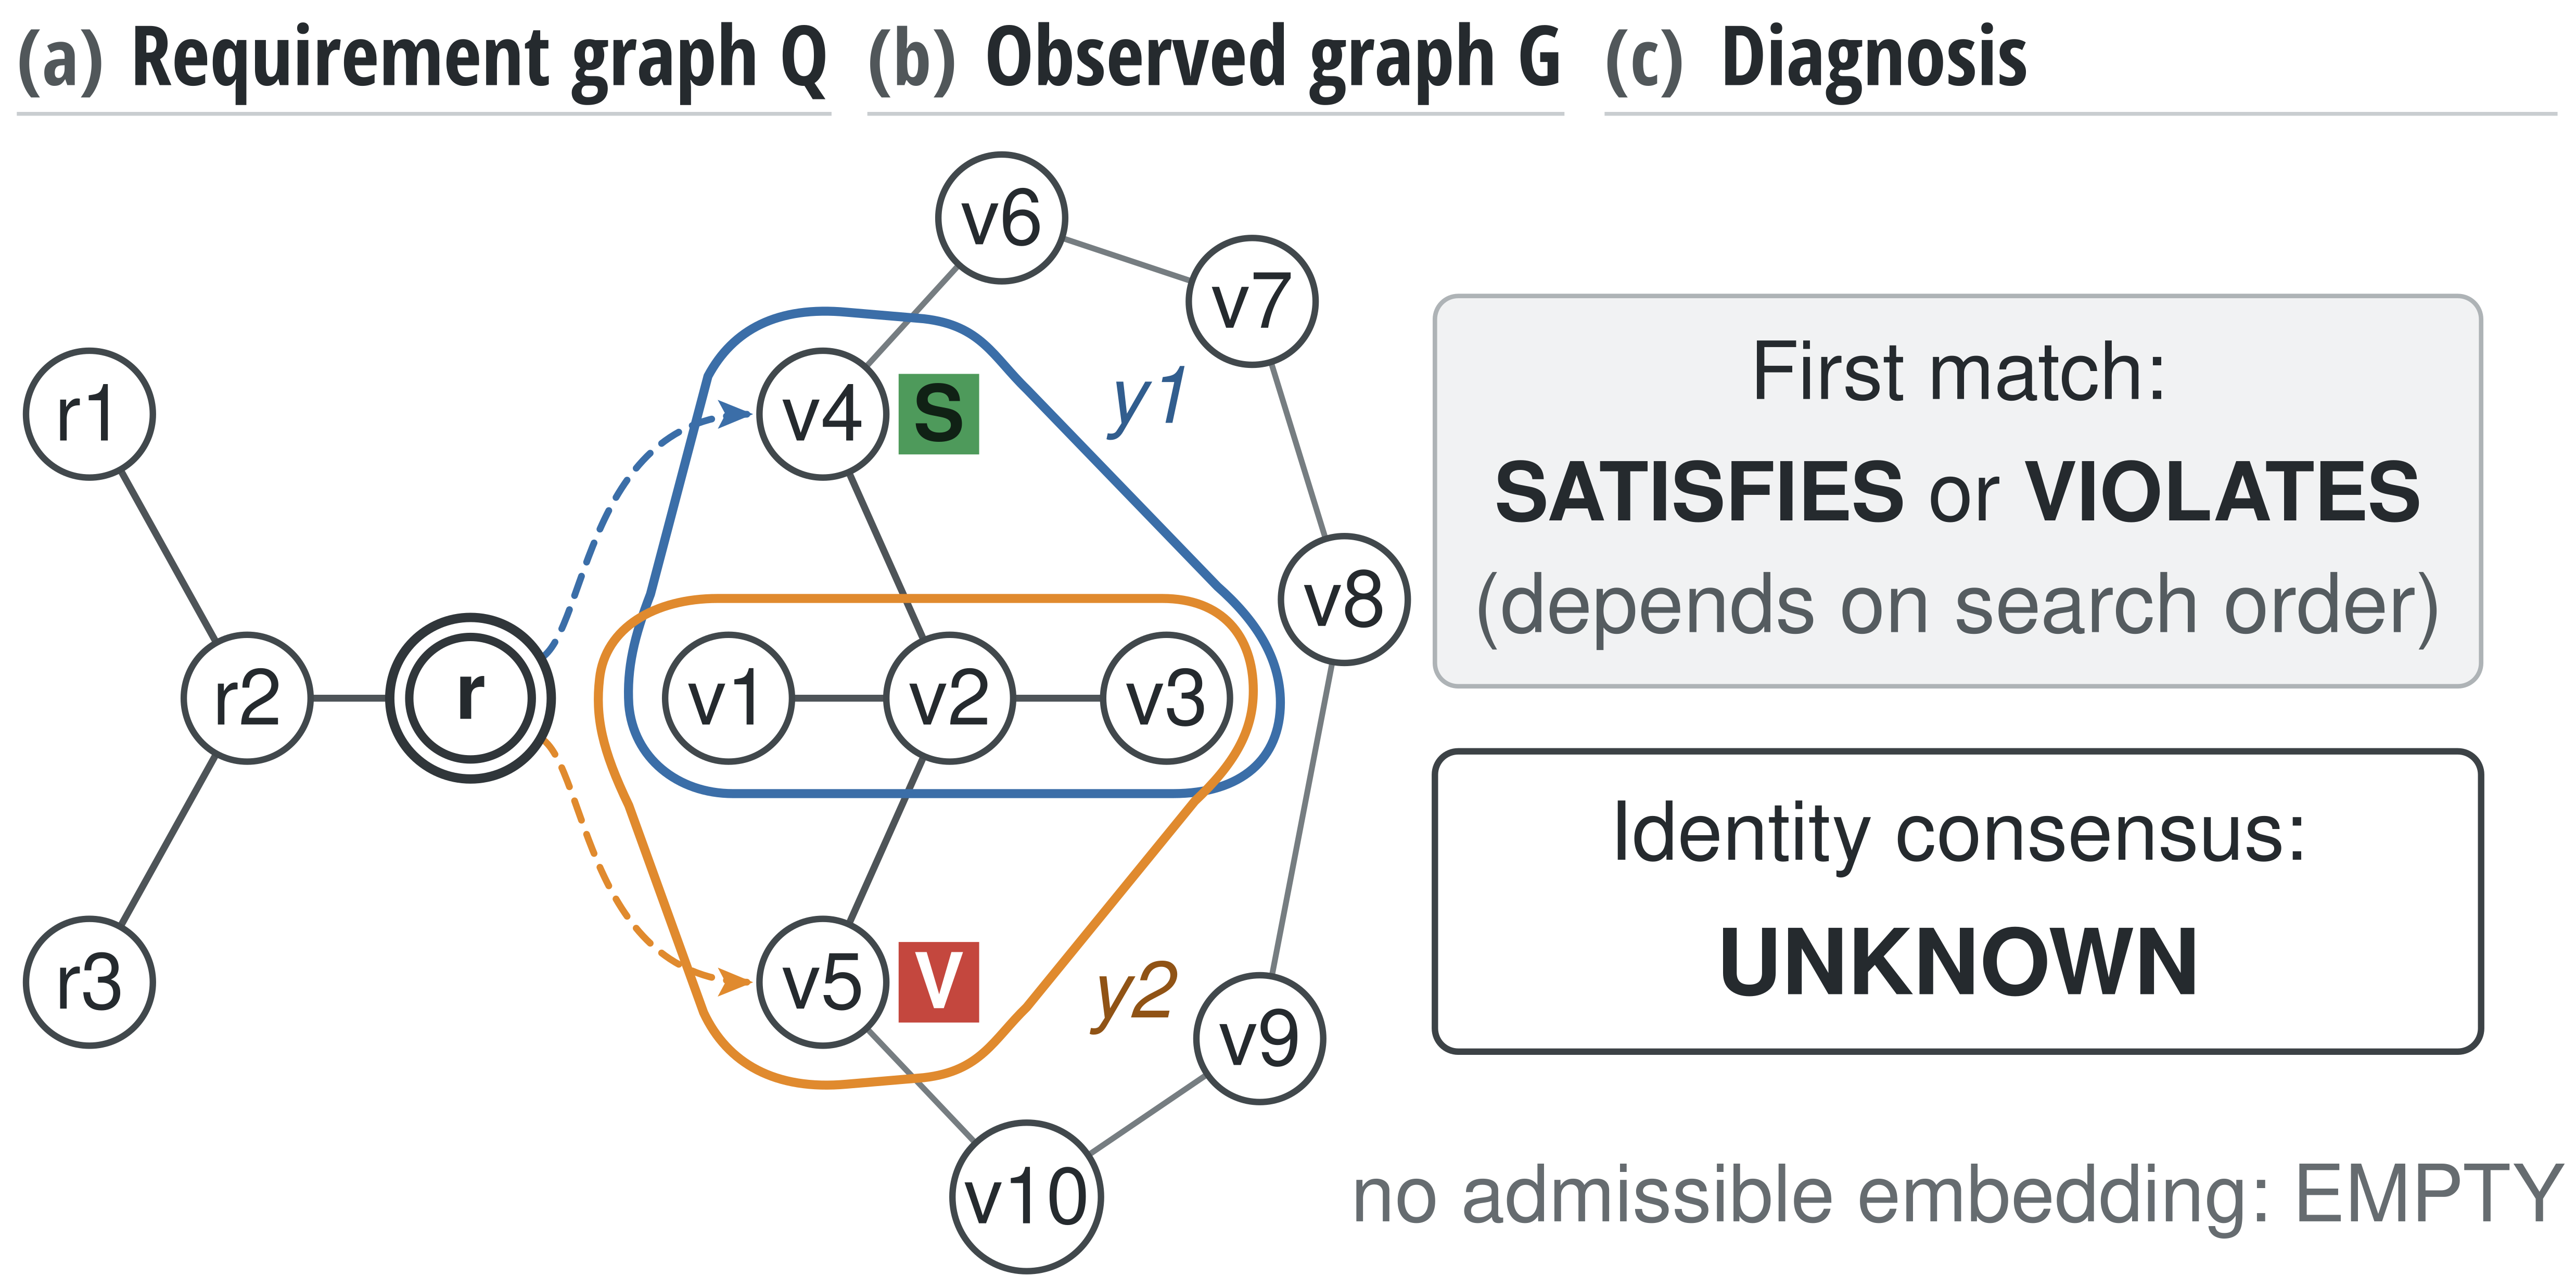
\includegraphics[width=\columnwidth]{figures/fig1_task.png}
\caption{Identity-consensus diagnosis. (a) Requirement graph $Q$ with checked role $r$. (b) Two admissible embeddings $y_1$ (blue) and $y_2$ (orange) in the observed graph $G$ agree on $r_1,r_2,r_3$ but place $r$ on an entity observed as $S$ and on one observed as $V$, respectively. (c) First-match diagnosis reports whichever embedding it finds first; the consensus answer is \Unk{}, and an empty identity space is reported as \Emp{}.}
\label{fig:task}
\end{figure}

\section{Related Work}
\textbf{Subgraph matching.} Exact matching is studied from Ullmann's backtracking \cite{ullmann} through VF2/VF3 \cite{cordella,vf3}, TurboISO \cite{turboiso}, verification-oriented filtering \cite{taming}, failing sets \cite{daf}, compact candidate spaces \cite{bice}, guard-based pruning \cite{gup}, decomposition \cite{asdmatch} and redundant-extension elimination \cite{cemr}; Sun and Luo \cite{sunluo} and RapidMatch \cite{rapidmatch} compare enumeration algorithms on shared query sets. Constraint-based engines such as LAD \cite{lad2010,lad} and the Glasgow Subgraph Solver \cite{glasgow} accept side constraints \cite{side_constraints}, can log proofs \cite{certified,e2everify,auditablecp}, and are combined in portfolios \cite{kotthoff}. Benchmarks for these systems measure the time to find one or all embeddings \cite{sunluo,mccreesh_hard}. IdCon asks a different question of the same engines: an aggregate over all embeddings, which enumeration answers only when the embeddings can be listed.

\textbf{Certain answers and consensus over solutions.} Asking which conclusions hold in every possible world is the certain-answer problem of incomplete databases \cite{imielinski,libkin2011,libkin2014}, studied for graph patterns over incomplete graphs \cite{barcelo}; consistent query answering asks it over the repairs of an inconsistent database \cite{arenas}, with systems that reduce it to integer programming \cite{equip} or SAT \cite{cavsat}, and explainable certain answers attach the witness that blocks a conclusion \cite{certain_answers}. In constraint reasoning the same question is the backbone of a formula \cite{backbones,cadiback} or the cautious consequences of an answer-set program \cite{cautious}, which clingo computes directly \cite{clingo}; IdCon includes both routes as baselines. Our possible worlds are injective, anchored, metric-respecting embeddings, which must be found by subgraph search (NP-hard even for one world \cite{karp,marx}), and the answer has four outcomes, so missing evidence ($U$), violation ($V$) and an empty world set stay distinct. Shape languages for knowledge graphs validate constraints per focus node, with partial assignments when recursion leaves truth values open \cite{shacl}; identity uncertainty in entity resolution is usually handled probabilistically \cite{pasula}, as is uncertain-graph matching with identity linkage \cite{moustafa}, whereas IdCon keeps identities deterministic and asks for consensus; model-based diagnosis \cite{reiter} infers faulty components, whereas IdCon takes observations as given.

\textbf{Benchmark practice.} We follow reproducibility guidance \cite{peng,gundersen,pineau}, document the data with a datasheet \cite{datasheets}, and report completion and penalized runtime as is standard for exact solvers \cite{mccreesh_hard}.

\section{Task}
\label{sec:task}
\textbf{Inputs.} A task consists of a pattern graph $Q=(R,E_Q)$ of roles, an observed graph $G=(N,E_G)$ of entities with coordinates $x:N\to\mathbb{R}^3$, an optional anchor map $a$ fixing some roles to entities, optional metric edges $(r,s,\ell)\in E_Q$ with tolerance $\epsilon$, optional unary domains $D_r\subseteq N$, a set of checked roles $R_c\subseteq R$ with observation tables $p_r:N\to\{S,U,V\}$, and a global state $t_0$, with order $S<U<V$.

\textbf{Identity space.} An admissible identity is an injective map $y:R\to N$ with $y(r)=a(r)$ for anchored roles, $y(r)\in D_r$, $\{y(r),y(s)\}\in E_G$ for every $\{r,s\}\in E_Q$, and $\bigl|\|x_{y(r)}-x_{y(s)}\|-\ell\bigr|<\epsilon$ for every metric edge. Extra observed edges are allowed (non-induced semantics). Let $\mathcal{Y}$ be the set of admissible identities and $T(y)=\max(t_0,\max_{r\in R_c}p_r(y(r)))$ the state of an identity.

\textbf{Outcomes.} The consensus answer is \Emp{} if $\mathcal{Y}=\emptyset$; \Sat{} if $T(y)=S$ for all $y\in\mathcal{Y}$; \Vio{} if $T(y)=V$ for all $y$; and \Unk{} otherwise, i.e., when some identity has state $U$ or the states disagree. A run that stops at its budget without a certified answer returns no answer.

\textbf{Two-query reduction.} Let $\exists(A)$ ask whether some $y\in\mathcal{Y}$ has $T(y)\in A$. Query $\exists(\{S,U,V\})$; a negative answer gives \Emp{}. If the witness has state $U$, the answer is \Unk{}. If it has state $s\in\{S,V\}$, query $\exists(\{S,U,V\}\setminus\{s\})$: a witness gives \Unk{}, a completed negative search gives \Sat{} or \Vio{}. Both queries are existential subgraph problems with unary restrictions: $T(y)\le h$ removes entities with $p_r>h$ from the domain of $r$, and $T(y)\ge l$ is a disjunction over checked roles. Any exact engine that accepts unary domains therefore becomes a consensus solver with at most two calls (or one per checked role for the disjunction), and every positive answer carries a replayable witness. The reduction is standard for certain answers; we state it because it fixes the interface of the IdCon adapters and locates the difficulty in the counterexample query, whose negative answer requires exhausting the search space.

\textbf{Example.} In Figure~\ref{fig:task} the first query may return $y_1$ with state $S$. The counterexample query then restricts $r$ to entities observed $U$ or $V$, finds $y_2$, and the answer is \Unk{}; had it returned $y_2$ first, it would find $y_1$. If $y_2$'s entity were observed $S$, the counterexample query would have to exhaust every identity that places $r$ on a non-$S$ entity before \Sat{} could be reported; a timeout there cannot be read as consensus, which is why IdCon scores unanswered runs separately.

\textbf{Complexity.} Deciding $\mathcal{Y}\neq\emptyset$ generalizes subgraph isomorphism, which contains CLIQUE \cite{karp}, and is NP-complete. \Unk{} is certified by at most two witnesses (an NP certificate); \Emp{} needs a refutation (coNP); \Sat{} and \Vio{} need both a witness and a refutation, so deciding them lies in DP.

\section{The IdCon Benchmark}
\label{sec:bench}
IdCon has five scored suites and two held-out splits (Table~\ref{tab:suites}). The independent unit is a graph-pair \emph{ancestor}: one pattern--host pair; observation tasks that share an ancestor are dependent, and the three HPRD suites share one host. Table~\ref{tab:suites} also reports three priors that predict the label without any search, from the scenario alone, from all metadata, and from a gradient-boosted classifier on metadata and observation-table statistics.

\begin{table*}[t]
\caption{IdCon suites. Labels: assessed references as \Sat/\Vio/\Unk/\Emp. Priors predict the label without search (leave one ancestor out): majority of the scenario, majority of all metadata, and a gradient-boosted classifier on metadata and observation-table statistics. IdCon-HPRD-H and IdCon-Hard-H are held-out splits whose labels are not public; IdCon-Hard-H inputs are also withheld (hashes published). $^\ddagger$: added in stage~3.}
\label{tab:suites}
\centering\footnotesize
\setlength{\tabcolsep}{3.5pt}
\begin{tabular}{lccccccc}
\toprule
 & Hard & Hard-X$^\ddagger$ & HPRD & HPRD-X & Cite$^\ddagger$ & HPRD-H & Hard-H$^\ddagger$\\
\midrule
Source & synthetic & synthetic & \multicolumn{2}{c}{HPRD; third-party queries} & Cora, PubMed & HPRD & synthetic\\
Ancestors / tasks & 72 / 504 & 12 / 72 & 100 / 200 & 96 / 192 & 96 / 192 & 100 / 200 & 12 / 72\\
Entities & 2,048--8,192 & 16,384 & 9,460 & 9,460 & 2,708; 19,717 & 9,460 & 16,384\\
Roles & 48--96 & 128 & 16 & 8--32 & 8--24 & 16 & 128\\
Anchors / metric & 0--2 / yes & 0--2 / yes & no / no & no / no & no / no & no / no & 0--2 / yes\\
Unary domains & no & no & yes & yes & yes & yes & no\\
Assessed refs & 504 & 68 & 200 & 192 & 192 & hidden & hidden\\
Labels & 171/128/161/44 & 21/9/30/8 & 16/99/85/0 & 19/93/80/0 & 14/52/126/0 & hidden & hidden\\
Scenario prior & 339/504 & 45/68 & 183/200 & 170/192 & 134/192 & -- & --\\
Metadata prior & 368/504 & 38/68 & 183/200 & 164/192 & 162/192 & -- & --\\
Learned prior & 419/504 & 52/68 & 181/200 & 166/192 & 162/192 & -- & --\\
\bottomrule
\end{tabular}
\end{table*}


\textbf{IdCon-Hard.} Each ancestor draws a host graph from one of six NetworkX families \cite{networkx} (random geometric, preferential attachment, small-world, random regular, Erd\H{o}s--R\'enyi, articulation modules) at one of three tiers (2,048/48, 4,096/64 or 8,192/96 entities/roles), extracts a pattern by seeded breadth-first search, and keeps either the induced subgraph or its BFS forest. A \emph{plain} variant has no anchors and no metric edges; a \emph{constrained} variant fixes the two highest-degree roles by coordinate and turns 30\% of pattern edges into metric edges on an integer coordinate grid, so that a metric edge prunes candidates without pinning the identity. The full factorial gives 72 ancestors. Eight non-anchored roles are checked. Observation scenarios place labels near the hidden construction embedding $y^*$: \emph{decoys} for a checked role $r$ are entities within one or two hops of $y^*(r)$ that $y^*$ does not use and that have sufficient degree, and a decoy matters exactly when some other admissible embedding maps $r$ there, a property of the graph rather than of the scenario. \textsf{decoy\_v} observes $y^*$ as $S$ and a random fraction of decoys as $V$; \textsf{decoy\_u} uses $U$ for the decoys; \textsf{focal\_v} observes one checked role as $V$ everywhere except at $S$ decoys; \textsf{mixed} combines $U$/$V$ decoys with sparse random violations; \textsf{background} marks a log-uniform fraction of all non-$y^*$ entities $V$; \textsf{perturbed} adds one to three required edges between roles at pattern distance two, which may or may not leave an admissible embedding; and \textsf{decoy\_s}, which turned out to be decided by the observation tables, is a control that the registered analysis keeps in the 504 scored tasks (Section~\ref{sec:prior} reports results without it). No solver is called during generation.

\textbf{IdCon-Hard-X and IdCon-Hard-H.} The same generator at 16,384 entities and 128 roles, with the six families crossed with forest/plain and induced/constrained (12 ancestors) and six scenarios (\textsf{decoy\_s} left out): \hardxTasks{} tasks. IdCon-Hard-H draws \hardhTasks{} tasks the same way with another seed; its inputs and references are not distributed, only their SHA-256 hashes. Its seed is in the released design record, so the split can be regenerated: like IdCon-HPRD-H it is held out by convention, for reporting results on tasks a method was not tuned on, and not a secret test set.

\textbf{IdCon-HPRD, -HPRD-X and -HPRD-H.} All three use the HPRD human protein interaction network as distributed by Sun and Luo \cite{sunluo,hprd} (9,460 entities, 34,998 edges, 307 vertex labels). \emph{IdCon-HPRD} uses the first 100 of their 200 dense 16-vertex query graphs; \emph{IdCon-HPRD-X} adds query graphs of 8, 16, 24 and 32 vertices, dense and sparse, from the public artifact of CEMR \cite{cemr} (12 per set, 96 ancestors); \emph{IdCon-HPRD-H} uses the other 100 Sun--Luo queries with undisclosed references. The benchmark adds two choices only: one to four seeded checked roles per query, and the observation rule. Unchecked roles keep their label as a unary domain; checked roles are free and observe $S$ where the matched entity carries the required label and $V$ otherwise. In \textsf{spec\_true} the required label is the query's own, asking whether the context forces the right protein at the checked positions; in \textsf{spec\_wrong} a different label is drawn by label frequency, modeling a misstated requirement.

\textbf{IdCon-Cite.} Cora (2,708 papers, 7 subject labels) \cite{cora} and PubMed (19,717 papers, 3 labels) \cite{pubmed} as distributed with Planetoid \cite{planetoid}, with their real topology and labels. Queries are extracted in the style of Sun and Luo: a seeded random walk collects $k\in\{8,16,24\}$ vertices and the induced subgraph is a dense (average degree $\ge 3$) or sparse query; 8 per set and host (96 ancestors). The observation rule is that of IdCon-HPRD. Few labels make the label domains wide, so this suite combines real structure with large identity spaces.

\textbf{Format and documentation.} Each task is a JSON identity (coordinates, host edges, role edges with optional lengths, anchors, optional unary domains) plus an observation table; construction maps are stored separately and read only by the reference builder. The release includes manifests with per-ancestor features, SHA-256 hashes of every input, the generators and importers, structural statistics (Appendix Table~\ref{tab:repr}) and a datasheet (Appendix~\ref{app:datasheet}).

\section{Evaluation Protocol}
\label{sec:protocol}
\textbf{References.} References are built by a process that never reads method predictions. For each task and state $s\in\{S,U,V\}$ we decide whether some identity has $T(y)=s$. States excluded by the observation tables are removed directly. The construction map, when admissible, is replayed against all original constraints and settles its own state. Remaining state queries run LAD2025 for 30~s; a LAD negative is re-checked by Glasgow for 30~s and marked \emph{confirmed} when Glasgow also completes; a LAD timeout falls back to Glasgow (60~s) and CP-SAT (60~s). Stage 2 re-queried every unconfirmed negative with Glasgow \texttt{-{}-staged} and CP-SAT and re-settled three IdCon-Hard tasks that stage 1 had settled with one of the authors' solvers (Appendix~\ref{app:registration}). Every positive witness is replayed by a checker. A task is assessed when its label is determined; others are \textsc{Unassessed} and excluded from every denominator. Method witnesses are replayed at scoring time; a replayed witness for a reference negative would invalidate the reference (none did).

\textbf{Independent check.} Because the reference engines are also benchmarked and share the adapters' encoding code, a separate check is written without any benchmark code: it reads the task JSON, encodes each exact-state query $T(y)=s$ in CNF (one-hot roles, at-most-one per entity, support clauses for pattern and metric edges) and solves it with CaDiCaL \cite{cadical}. A witness is replayed against the raw input; a negative is re-derived on the encoding without any pruning and accepted only with a DRAT proof verified by drat-trim \cite{drattrim}. It runs on every IdCon-Hard task with an unconfirmed negative, on 48 stratified random IdCon-Hard tasks, on the IdCon-HPRD-X tasks that ASP-cautious did not answer, on every IdCon-Cite task, and on IdCon-Hard-X on one task per ancestor plus every task with a negative that only one reference engine established. The design record checked every IdCon-Hard-X task with 600\,s per solve; two amendments made during the runs lowered the limits to 120\,s and replaced full coverage of IdCon-Hard-X by this selection, because the check would not have finished on the machine (Appendix~\ref{app:registration}).

\textbf{Methods.} All methods receive the same JSON input and run end to end, including parsing, encoding and process launch, under a 2-second budget on one thread. Two-query adapters (Section~\ref{sec:task}): \emph{LAD} runs LAD2025 \cite{lad} patched to accept unary domains and metric-edge lists; \emph{Glasgow} encodes domains and metric edges as labeled pendant gadgets for the Glasgow Subgraph Solver \cite{glasgow}, whose labelled formats cannot leave some pattern vertices unconstrained; \emph{Glasgow-staged} adds its \texttt{-{}-staged} preprocessing (post hoc on IdCon-Hard and IdCon-HPRD, marked $^\dagger$); \emph{CP-SAT} and \emph{Trad-CP} model identities with AllDifferent and table constraints in OR-Tools. Enumerate-and-aggregate: \emph{Enum-Glasgow} and \emph{Enum-VF2} \cite{networkx,cordella} list identities and stop as soon as two disagree or one has state $U$. Certain-answer reasoning: \emph{ASP-cautious} asks clingo \cite{clingo} for the cautious consequences of $T$; \emph{SAT}$^\ddagger$ runs the two-query reduction on the CNF encoding above with one CaDiCaL process per query. Methods added in stage 2 are marked $^\ast$, those added in stage 3 $^\ddagger$. \emph{First-match} runs one LAD query and reports the state of the first identity.

\textbf{Scoring.} A run is \emph{correct} when its outcome equals the reference. We report correct runs; wrong runs; ancestor-equal PAR-2 (rows averaged within an ancestor, then across ancestors), which charges 4~s for an unanswered or wrong run; and, for uncertified methods, PAR-2 with a 20~s charge per wrong run (PAR-10w). A method that returns a certified outcome contradicting a reference is \emph{unsound} and is not ranked by runtime. The virtual best solver (VBS) takes, per run, any sound method that answers it; we state each time which methods it includes. Strata are compared with ancestor-level bootstrap (10,000 draws), reporting how often a method is best and the interval of its difference to the runner-up; when that interval includes 0 we call the two methods not distinguishable. Each task is run twice per method in a randomized order on a 2-vCPU VM in stages 1 and 2; stage 3 ran on a different 2-vCPU VM that is \calibRatio{} times slower on IdCon-Hard (median ratio over \calibBoth{} runs answered on both machines; \calibAgree{} of \calibRuns{} outcomes agree).

\textbf{Stages and registration.} The study ran in three stages. Stage~1 built IdCon-Hard and IdCon-HPRD and ran LAD, Glasgow, CP-SAT, Trad-CP, first-match and two solvers of the authors; stage~2 added IdCon-HPRD-X, IdCon-HPRD-H, the stage-2 methods and the 10\,s reruns, and dropped the authors' solvers from the benchmark; stage~3 added IdCon-Hard-X, IdCon-Hard-H, IdCon-Cite, SAT, the independent check and the 60\,s reruns. Each stage fixed seeds, factors, methods, budgets, scoring and reference procedure in a hash-stamped design record before its runs; the records and their amendments are released, but their times are the authors' own and not certified by a third party. Several stage-2 and stage-3 analyses were fixed after stage-1 results on the same suites were known; Appendix Table~\ref{tab:registration} says, for every reported analysis, when it was fixed and whether results on the same data were known then.

\section{Results}
\label{sec:results}
\begin{table*}[t]
\caption{Main results under the 2\,s end-to-end budget (two repeats per task). Correct: outcome equals the reference. Wrong: answered but different from the reference; for a certified answer this is a soundness failure (none occurred). PAR-2: ancestor-equal mean, 4\,s for an unanswered or wrong run; best certified method per suite in bold. PAR-10w charges a wrong answer 20\,s instead (it differs from PAR-2 only for uncertified methods). $^\ast$added in stage~2; $^\ddagger$SAT encoding solved by CaDiCaL, added in stage~3; $^\dagger$post hoc arm on Hard and HPRD. Priors predict labels without search, leave one ancestor out, counted per run.}
\label{tab:main}
\centering\small\setlength{\tabcolsep}{4.5pt}
\begin{tabular}{l rrr rrr rrr}
\toprule
 & \multicolumn{3}{c}{IdCon-Hard (1,008 runs)} & \multicolumn{3}{c}{IdCon-HPRD (400 runs)} & \multicolumn{3}{c}{IdCon-HPRD-X (384 runs)}\\
\cmidrule(lr){2-4}\cmidrule(lr){5-7}\cmidrule(lr){8-10}
Method & Correct & Wrong & PAR-2 & Correct & Wrong & PAR-2 & Correct & Wrong & PAR-2\\
\midrule
LAD & 725 & 0 & \textbf{1,635} & 389 & 0 & 1,036 & 199 & 0 & 2,513\\
Glasgow & 562 & 0 & 2,113 & 0 & 0 & 4,000 & 1 & 0 & 3,995\\
Glasgow-staged$^\dagger$ & 651 & 0 & 1,740 & 304 & 0 & 1,361 & 265 & 0 & 1,734\\
CP-SAT & 321 & 0 & 2,998 & 384 & 0 & 455 & 360 & 0 & 830\\
Trad-CP & 214 & 0 & 3,347 & 279 & 0 & 1,858 & 191 & 0 & 2,603\\
Enum-Glasgow$^\ast$ & 88 & 0 & 3,688 & 235 & 0 & 2,638 & 65 & 0 & 3,568\\
Enum-VF2$^\ast$ & 14 & 0 & 3,951 & 127 & 0 & 2,937 & 74 & 0 & 3,354\\
ASP-cautious$^\ast$ & 15 & 0 & 3,968 & 400 & 0 & 748 & 365 & 0 & 1,230\\
SAT$^\ddagger$ & 240 & 0 & 3,378 & 400 & 0 & \textbf{374} & 384 & 0 & \textbf{380}\\
\midrule
First-match (PAR-2 / PAR-10w) & 626 & 315 & 1,901 / 6,901 & 230 & 170 & 2,027 / 8,827 & 224 & 160 & 2,242 / 8,909\\
Metadata prior & 736 & 272 & -- & 366 & 34 & -- & 328 & 56 & --\\
Learned prior & 838 & 170 & -- & 362 & 38 & -- & 332 & 52 & --\\
\bottomrule
\end{tabular}
\end{table*}


\subsection{Embeddings are rarely unique; first-match is wrong where they disagree}
\label{sec:firstmatch}
What carries over to other workloads is how often embeddings are not unique, which does not depend on our observation rule. Counting embeddings with Glasgow (30~s per query), \hprdCountFullMulti{} of the \hprdCountFullQueries{} IdCon-HPRD queries have more than one embedding when every query vertex must match its own label, and \hprdAutoOrbitMulti{} still do after dividing by the number of label-preserving automorphisms of the query, i.e., counting genuinely different placements (\hprdCountFullThousand{} queries have at least 1,000 embeddings; no count hit the time limit); on IdCon-HPRD-X the figures are \hprdxCountFullMulti{} and \hprdxAutoOrbitMulti{} of \hprdxCountFullQueries{}. With the checked roles freed, \hprdCountSpaceMulti{} and \hprdxCountSpaceMulti{} of the identity spaces have more than one identity.

A first match can be wrong only on an \Unk{} task: if the reference is \Sat{} or \Vio{} every identity has that state, and if it is \Emp{} there is nothing to report. Every wrong first-match run in IdCon is indeed on an \Unk{} task (\hardFirstWrongOnUnknown{} of \hardFirstWrong{} on IdCon-Hard, \hprdFirstWrongOnUnknown{} of \hprdFirstWrong{} on IdCon-HPRD, \hprdxFirstWrongOnUnknown{} of \hprdxFirstWrong{} on IdCon-HPRD-X; Table~\ref{tab:main}). Its error rate on a suite is therefore the share of tasks whose embeddings disagree, a property of the workload rather than a finding: \hardFirstWrongAnsweredPct\% of answered IdCon-Hard runs, set by the generator's decoy rates, and \hprdFirstWrongPct\% of IdCon-HPRD runs, set by the observation rule (\hprdFirstWrongSpecTrue{} of the \hprdFirstWrong{} wrong runs are \textsf{spec\_true} tasks).

\subsection{Exact methods are sound, and none dominates}
\label{sec:exact}
No exact method returned a certified outcome that contradicts a reference on any suite, and all \witnessTotalRtwo{} positive witnesses returned by methods on the five scored suites replay against the original constraints. On IdCon-Hard, \hardBest{} has the lowest PAR-2 (\hardBestPar~ms; runner-up \hardSecond{}, \hardSecondPar~ms). On IdCon-HPRD and IdCon-HPRD-X, \hprdBest{} and \hprdxBest{} have (\hprdBestPar{} and \hprdxBestPar~ms; runners-up \hprdSecond{} and \hprdxSecond{}, \hprdSecondPar{} and \hprdxSecondPar~ms), and \hprdMost{} and \hprdxMost{} answer the most runs (\hprdMostCorrect{} of \hprdASPcautiousAssessed{} and \hprdxMostCorrect{} of \hprdxASPcautiousAssessed{}). The SAT baseline thus leads where label domains are narrow, yet answers only \hardSATCorrect{} of \hardSATAssessed{} IdCon-Hard runs, where its encoding grows with the number of candidates per role. Inside the suites the best method changes with size, anchoring and query size (Appendix Figure~\ref{fig:strata} and Tables~\ref{tab:strata-hard}--\ref{tab:strata-hprdx}); with the share of bootstrap resamples in which it stays best in brackets, and n.s.\ where it is not distinguishable from the runner-up, \strataSentence{}. With 12 ancestors per IdCon-Hard stratum these comparisons are coarse. At 2\,s the best single method leaves \hardBestUnsolvedPct\% of IdCon-Hard runs unsolved; a VBS over the methods registered in stages 1 and 2 (Glasgow-staged excluded as a post hoc arm) leaves \hardVBSUnsolved{} runs (\hardVBSUnsolvedPct\%), and one over every sound method including Glasgow-staged and SAT leaves \hardVBSAllUnsolved{} (\hardVBSAllUnsolvedPct\%). These figures describe the benchmarked methods at 2\,s, not a limit of exact methods: two unpublished solvers of the authors, run in stage~1 and not part of the benchmark, answer \legEgCorrect{} and \legSvCorrect{} of the 1,008 IdCon-Hard runs at 2\,s, and with them the VBS leaves \legVBSBoth{} (Appendix Table~\ref{tab:legacy}).

\begin{table}[t]
\caption{Stage-3 suites (repeat~0, one run per task and budget on IdCon-Hard-X; two repeats at 2\,s on IdCon-Cite). Correct runs within 2, 10 and 60\,s (a run unanswered at a budget is rerun at the next for the methods listed in the design record; -- not rerun). VBS: tasks that no sound method answers within the budget. No certified answer contradicts a reference.}
\label{tab:newsuites}
\centering\footnotesize
\setlength{\tabcolsep}{2.6pt}
\begin{tabular}{lrrr rrr}
\toprule
 & \multicolumn{3}{c}{IdCon-Hard-X (68 tasks)} & \multicolumn{3}{c}{IdCon-Cite (192 tasks)}\\
\cmidrule(lr){2-4}\cmidrule(lr){5-7}
Method & 2\,s & 10\,s & 60\,s & 2\,s$^{2}$ & PAR-2 & 10\,s\\
\midrule
LAD & 1 & 30 & 64 & 192 & 2,086 & 191\\
Glasgow & 1 & 29 & -- & 92 & 3,256 & --\\
Glasgow-staged & 15 & 33 & 46 & 126 & 2,904 & 107\\
CP-SAT & 5 & 11 & -- & 124 & 2,911 & 88\\
Trad-CP & -- & -- & -- & 190 & 2,188 & --\\
Enum-Glasgow$^\ast$ & 1 & 4 & -- & 104 & 3,118 & --\\
Enum-VF2$^\ast$ & -- & -- & -- & 77 & 3,300 & --\\
ASP-cautious$^\ast$ & -- & -- & -- & 223 & 1,964 & 192\\
SAT$^\ddagger$ & 2 & 2 & 40 & 265 & 1,598 & 192\\
\midrule
First-match & 1 & 35 & -- & 114 & 2,837 & --\\
\midrule
VBS unsolved & 49 & 23 & 3 & 110 & -- & 0\\
\bottomrule
\end{tabular}
\end{table}


\subsection{Larger hosts and real labels}
\label{sec:newsuites}
The stage-3 suites change the picture where IdCon-Hard is near saturation (Table~\ref{tab:newsuites}). On IdCon-Hard-X, where one LAD2025 query alone takes about 3\,s on a 16,384-entity host, the methods jointly leave \hardxVBSUnsolvedTwo{} of \hardxComplete{} assessed tasks unanswered at 2\,s, \hardxVBSUnsolvedTen{} at 10\,s and \hardxVBSUnsolvedSixty{} at 60\,s; the best single method answers \hardxBestSingleTenN{} within 10\,s (\hardxBestSingleTen{}) and \hardxBestSingleSixtyN{} within 60\,s (\hardxBestSingleSixty{}). Glasgow-staged answers most at 2\,s, LAD after its slow first query. On IdCon-Cite, whose few labels leave wide domains on real citation graphs, the fastest sound method is \citeBest{} (PAR-2 \citeBestPar~ms), the certain-answer formulations (ASP-cautious, SAT) are competitive with the two-query adapters, and the methods jointly leave \citeVBSUnsolvedRuns{} of the 2\,s runs unanswered and \citeVBSUnsolvedTen{} tasks at 10\,s. No certified answer contradicts a reference on either suite.

\begin{figure*}[t]
\centering
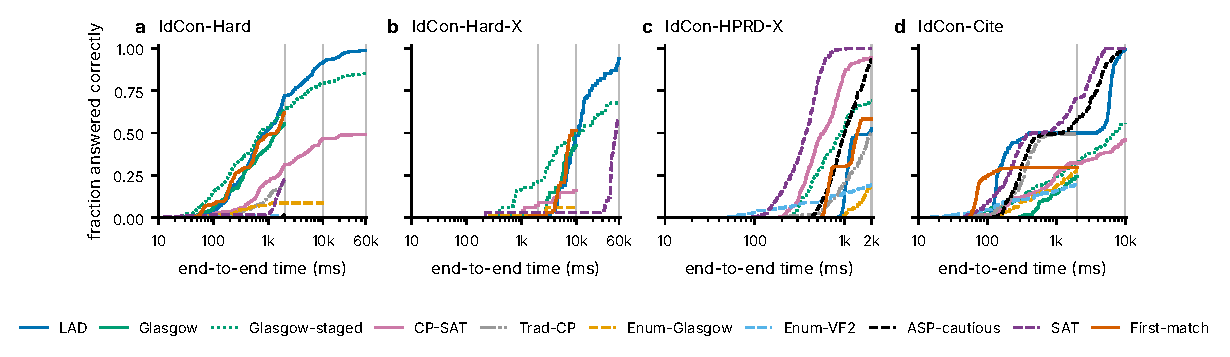
\includegraphics[width=\textwidth]{figures/fig2_results.pdf}
\caption{Fraction of assessed tasks answered correctly within a given end-to-end time (repeat~0). Runs unanswered at 2\,s continue with the 10\,s rerun and, for the methods rerun at 60\,s, with the 60\,s rerun (grey lines: 2, 10 and 60\,s). (a) IdCon-Hard, (b) IdCon-Hard-X, (c) IdCon-HPRD-X, (d) IdCon-Cite. Dashed: methods added in stages 2 and 3. Times after the first budget on IdCon-Hard come from the stage-3 machine (\calibRatio{} times slower).}
\label{fig:results}
\end{figure*}

\subsection{Budget, overhead and headroom}
\label{sec:budget}
The difficulty of IdCon-Hard is largely a 2\,s difficulty (Figure~\ref{fig:results}a). On repeat~0, LAD answers \hardLadRepTwo{} of 504 tasks at 2\,s, \hardLadRepTen{} at 10\,s and \hardLadRepSixty{} at 60\,s; the VBS over every sound method leaves \hardVBSAllUnsolvedTwo{}, \hardVBSAllUnsolvedTen{} and \hardVBSAllUnsolvedSixty{} tasks unanswered (at 60\,s: \hardVBSSixtyLabels{}). IdCon-Hard therefore separates methods at short budgets and is close to solved with a minute per task; IdCon-Hard-X separates them at 10\,s (Section~\ref{sec:newsuites}). On IdCon-HPRD every method rerun at 10\,s reaches at least \hprdGlasgowTenS{} of \hprdRepZeroN{} tasks, and ASP-cautious and SAT answer \hprdASPcautiousCorrect{} and \hprdSATCorrect{} of its \hprdSATAssessed{} runs at 2\,s; that suite's 2\,s ranking measures per-call start-up cost more than search. The cost is visible directly. On IdCon-HPRD one LAD call on a one-role pattern takes \ovhLadOneRole~ms end to end and one default Glasgow call \ovhGlasgowOneRole~ms. On 48 stratified IdCon-Hard tasks, the first LAD query takes \ovhHardLadTotal~ms (median), of which \ovhHardLadOutside~ms are spent outside the solver process (building the graph, writing files) and the solver process \ovhHardLadSolver~ms; for Glasgow-staged the figures are \ovhHardGSTotal, \ovhHardGSOutside{} and \ovhHardGSSolver~ms. Results at one budget should be read with the completion curves, and adapter engineering is part of what the 2\,s budget measures.

\subsection{Tools and universal outcomes}
\label{sec:tools}
On IdCon-Hard, where by degree almost every entity is a candidate for every role, enumeration and grounding do not finish: Enum-Glasgow answers \hardEnumGlasgowCorrect{}, Enum-VF2 \hardEnumVFTwoCorrect{} and ASP-cautious \hardASPcautiousCorrect{} of \hardEnumGlasgowAssessed{} runs. Where label domains are narrow (HPRD) the certain-answer formulations are the most complete methods: ASP-cautious and SAT answer \hprdxASPcautiousCorrect{} and \hprdxSATCorrect{} of the \hprdxSATAssessed{} IdCon-HPRD-X runs. \Unk{} needs witnesses only, whereas \Sat{}, \Vio{} and \Emp{} need a completed negative search, and the methods differ most on the latter: on IdCon-Hard, LAD answers \hardLADSatCorrect{} \Sat{} runs and CP-SAT \hardCPSATSatCorrect{}, against \hardLADUnkCorrect{} and \hardCPSATUnkCorrect{} \Unk{} runs (Appendix Table~\ref{tab:labels}).

\subsection{What can be predicted without search}
\label{sec:prior}
On IdCon-Hard the scenario alone predicts \hardPriorScenario{} references, all metadata \hardPriorMeta{}, and the learned prior \hardPriorLearned{} (\hardPriorLearnedPct\%); \priorWrongAllThree{} references defeat all three priors. Two shortcuts explain much of this. First, in \sensDecided{} tasks (\sensDecidedPct\%; \sensDecidedDecoyS{} of them the \textsf{decoy\_s} control) the observation tables exclude two of the three states in a scenario whose construction embedding is admissible, so one existence query decides the label; a method that adds this table check gains these runs. Second, on the HPRD suites the scenario fixes the label for \hprdPriorScenario{} and \hprdxPriorScenario{} tasks, because a misstated label is rarely carried by an admissible embedding. The ranking of the exact methods is robust to both: without \textsf{decoy\_s} and without all \sensDecided{} table-decided tasks, \sensRankSentence{} (post hoc, Appendix Table~\ref{tab:sensitivity}). On IdCon-Hard-X and IdCon-Cite the learned prior reaches \hardxPriorLearned{} and \citePriorLearned{}. A learned predictor has to beat these numbers before its accuracy reflects the graph; for exact methods the shortcuts only mean that part of a suite is easy. Because the released tools compute exact labels from public inputs (IdCon-HPRD-H) or from a public seed (IdCon-Hard-H), the held-out splits guard against tuning, not against a determined user.

\begin{table}[t]
\caption{Independent reference check: an encoding written without any benchmark code, solved by CaDiCaL; witnesses replayed against the raw input; negatives decided on the unpruned encoding with DRAT proofs verified by drat-trim. Settles: tasks \textsc{Unassessed} in the reference that the check decides. Limits: 600\,s per solve and 1,200\,s per proof check (registered) for the first 4 tasks, 120\,s and 300\,s for the rest (Amendment~6); Hard-X single-engine negatives: every IdCon-Hard-X task with a negative state that only one reference engine established, not already sampled (Amendment~7).}
\label{tab:idcheck}
\centering\footnotesize
\setlength{\tabcolsep}{3pt}
\begin{tabular}{lrrrrr}
\toprule
Sample & Tasks & Agree & Disagree & Unresolved & Settles\\
\midrule
Hard, unconfirmed negative & 17 & 10 & 0 & 7 & 0\\
Hard, stratified random & 48 & 44 & 0 & 4 & 0\\
HPRD-X, no ASP answer & 4 & 4 & 0 & 0 & 0\\
Cite, all tasks & 192 & 192 & 0 & 0 & 0\\
Hard-X, one per ancestor & 12 & 10 & 0 & 1 & 1\\
Hard-X, single-engine negative & 19 & 19 & 0 & 0 & 0\\
\midrule
Total & 292 & 279 & 0 & 12 & 1\\
\bottomrule
\end{tabular}
\end{table}


\subsection{Reference quality}
\label{sec:refquality}
Every positive state is a replayed witness. Of the \hardNegRone{} non-trivial IdCon-Hard negatives, \hardNegRoneCorroborated{} are confirmed by a second engine after the stage-2 re-check (\hardNegVoneCorroborated{} of \hardNegVone{} after stage~1); on IdCon-HPRD all \hprdNegRone{} are, and on IdCon-HPRD-X \hprdxNegRoneCorroborated{} of \hprdxNegRone{}. The second engines are themselves benchmarked and share the adapters' code, so we added the independent check of Section~\ref{sec:protocol} (Table~\ref{tab:idcheck}): it decides \idcDecided{} of \idcTasks{} sampled and new-suite tasks, agrees with \idcAgree{} references, contradicts \idcDisagree{} and decides \idcSettles{} that the reference procedure left \textsc{Unassessed} (\idcUnresolved{} unresolved; \idcDrat{} negative states carry verified DRAT proofs), including \idcUnconfAgree{} of the \idcUnconfTasks{} IdCon-Hard tasks whose negatives no second engine had confirmed. The new suites need it most on IdCon-Hard-X, where Glasgow corroborates only \hardxNegCorroborated{} of \hardxNeg{} non-trivial negatives within its 30\,s on the 16,384-entity hosts (IdCon-Cite: \citeNegCorroborated{} of \citeNeg{}); the check agrees on \idcHardxSingleAgree{} of the \idcHardxSingleTasks{} IdCon-Hard-X tasks with such a single-engine negative (\idcHardxSingleUnresolved{} unresolved) and on \idcCiteAgree{} of \idcCiteTasks{} IdCon-Cite tasks. Restricted to fully confirmed references, the ranking of the sound methods \refRankSentence{} (Appendix Table~\ref{tab:refs}).


\section{Using IdCon}
\textbf{Interface.} A method receives the identity record, the observation tables and a budget, and returns an outcome, a certificate flag and every positive witness it found. The driver measures the full call; nothing in it gives a method access to construction maps or references. Adding a method needs one adapter function and one dispatch line.

\textbf{What to report.} Per suite: correct, wrong and unanswered runs; ancestor-equal PAR-2; correct runs by reference label (Appendix Table~\ref{tab:labels}), because a method that only finds witnesses looks strong on \Unk{} and weak elsewhere; completion curves to at least 60\,s; and the number of certified outcomes that disagree with the reference, which must be zero for an exact method. Approximate and learned methods leave the certificate flag unset and must beat the learned prior of Table~\ref{tab:suites}. Predictions on the held-out splits are scored by the maintainers.

\textbf{Extending IdCon.} The generator exposes its factors (family, tier, density, construction, anchors, metric fraction, scenario parameters) and is deterministic given a seed; harder tiers can be added without touching existing records, as IdCon-Hard-X shows. A new population should be registered before it is run and should report its no-search priors.

\section{Reproducibility and Release}
The release contains, per suite, the generator or importer, input hashes, protected construction maps, references with their engine logs, frozen predictions, the independent checker, scoring code and a read-only verifier that recomputes every table and number of this paper from the frozen records. Adapters, the patched LAD2025 sources (CeCILL-B) and build scripts are included; Glasgow, CaDiCaL, drat-trim, clingo, NetworkX and OR-Tools are obtained upstream with versions and hashes recorded. Project code is MIT and our generated data, references and predictions are CC BY 4.0, at \url{\repourl}. HPRD is free for academic, non-commercial use only, the CEMR query files carry no licence, and Cora and PubMed are taken from the MIT-licensed Planetoid repository; none is redistributed: scripts fetch them from pinned upstream commits and check their hashes, and task files built from them are generated locally. Rebuilt binaries reproduce labels, not timings.

\section{Limitations and Ethics}
\label{sec:limits}
The synthetic suites are not samples of engineering requirement graphs; the HPRD and Cite suites supply real topology and labels with our checked-role choice and observation rule, so observations are label agreement rather than measured defects. No suite comes from a deployed requirement-checking system. Negative references are solver-trusted except where the independent check verified a DRAT proof; we report confirmation rates and results restricted to confirmed references. Methods that launch external processes pay that cost per query, in-process methods do not, and the 2\,s budget measures that cost as well as search (Section~\ref{sec:budget}); budgets are enforced by killing solver processes and by time checks in Python-side encoding, so an encoding phase can overrun (scored as unanswered). Timings come from two 2-vCPU VMs with two concurrent single-thread processes; the two repeats agree on \hardRepeatAgreePct\% (Hard), \hprdRepeatAgreePct\% (HPRD) and \hprdxRepeatAgreePct\% (HPRD-X) of outcomes, the last because many HPRD-X runs finish close to the budget. The two solvers run in stage~1 and then left out of the benchmark are the authors' own unpublished methods; their results are disclosed (Appendix Table~\ref{tab:legacy}) but not ranked.

The benchmark contains no personal data. A consensus checker can make an engineering or biological check stricter; it cannot certify that the requirement graph itself is right, and \Sat{} should not be read as validation of the requirement.

\section{Discussion}
\textbf{For practitioners.} The shortcut is safe only when the admissible embedding is unique, and on the third-party queries it rarely is (Section~\ref{sec:firstmatch}). A cheap safeguard follows from the reduction: after a first match, issue the counterexample query. If it completes without a witness, the first-match answer was right; if it finds one, the answer is \Unk{}; if it times out, report the result as undetermined rather than as the first-match label.

\textbf{For solver designers.} The suites reward different engines: LAD's propagation on large unanchored ambiguous patterns, Glasgow's staged preprocessing on the largest hosts, and SAT and cautious reasoning when label domains are narrow or the identity space is small enough to ground; whole-model CP wins some anchored strata. IdCon-Hard is a short-budget suite: with a minute per task the benchmarked methods jointly leave \hardVBSAllUnsolvedSixty{} of its 504 tasks open, and unpublished methods already do better at 2\,s (Appendix Table~\ref{tab:legacy}). IdCon-Hard-X moves the separating budget up: within 10\,s the best single method answers \hardxBestSingleTenN{} of its \hardxComplete{} assessed tasks and all methods together leave \hardxVBSUnsolvedTen{} open, while \hardxBestSingleSixty{} answers \hardxBestSingleSixtyN{} with 60\,s. IdCon-Cite is a 2\,s suite: some method answers every task within 10\,s, but at 2\,s the best single method answers \citeBestSingleTwoN{} of \citeTasks{}. None of the suites is beyond exact search with a minute per task, so IdCon measures the cost of exact consensus rather than its feasibility; the released generator scales further. The hardest outcomes are the universal ones, where proving \Sat{} requires refuting every non-$S$ placement; the independent check shows that DRAT proofs for such refutations are practical for many IdCon instances, so proof-producing consensus solvers \cite{auditablecp} can be held to certified negatives.


\section{Conclusion}
IdCon makes identity-consensus diagnosis measurable. Admissible embeddings are rarely unique in third-party query workloads, even up to query symmetry, so a match-then-read check is wrong wherever they disagree; how often that happens is a property of the workload. Exact consensus is sound with every engine we tried, and no engine dominates: two-query adapters, whole-model CP, enumeration, cautious reasoning and SAT each win somewhere and fail somewhere else. How hard the benchmark is depends on the budget and the suite: IdCon-Hard and IdCon-Cite separate methods at 2\,s, IdCon-Hard-X at 10\,s, and with a minute per task the methods together answer nearly every task, so what IdCon measures is the cost of exact consensus. The benchmark fixes the interface, references with an independent proof-checked sample, scoring, and two held-out splits, so that new consensus engines, including proof-producing and learned ones, can be compared directly.



\begin{acks}
\textbf{Generative AI disclosure.} An AI assistant (Claude, Anthropic) was used under the authors' direction to write and refactor experiment code (including the SAT baseline, the independent checker and the analysis scripts), to run experiments, and to draft and revise text. The authors specified the study, reviewed all code, results and text, and take full responsibility for the content. Funding acknowledgments will be added for the camera-ready version.
\end{acks}

\begin{thebibliography}{99}
\bibitem{imielinski} Tomasz Imieli\'nski and Witold Lipski. 1984. Incomplete information in relational databases. \textit{Journal of the ACM} 31(4), 761--791. \url{https://doi.org/10.1145/1634.1886}
\bibitem{libkin2014} Leonid Libkin. 2014. Incomplete data. In \textit{PODS 2014}, 1--13. \url{https://doi.org/10.1145/2594538.2594561}
\bibitem{ullmann} Julian R. Ullmann. 1976. An algorithm for subgraph isomorphism. \textit{Journal of the ACM} 23(1), 31--42. \url{https://doi.org/10.1145/321921.321925}
\bibitem{cordella} Luigi P. Cordella, Pasquale Foggia, Carlo Sansone, and Mario Vento. 2004. A (sub)graph isomorphism algorithm for matching large graphs. \textit{IEEE Transactions on Pattern Analysis and Machine Intelligence} 26(10), 1367--1372. \url{https://doi.org/10.1109/TPAMI.2004.75}
\bibitem{vf3} Vincenzo Carletti, Pasquale Foggia, Alessia Saggese, and Mario Vento. 2017. Introducing VF3: A new algorithm for subgraph isomorphism. In \textit{GbRPR 2017}, 128--139. \url{https://doi.org/10.1007/978-3-319-58961-9_12}
\bibitem{turboiso} Wook-Shin Han, Jinsoo Lee, and Jeong-Hoon Lee. 2013. TurboISO: Towards ultrafast and robust subgraph isomorphism search in large graphs. In \textit{SIGMOD 2013}, 337--348. \url{https://doi.org/10.1145/2463676.2465300}
\bibitem{taming} Haichuan Shang, Ying Zhang, Xuemin Lin, and Jeffrey Xu Yu. 2008. Taming verification hardness: An efficient algorithm for testing subgraph isomorphism. \textit{PVLDB} 1(1), 364--375. \url{https://doi.org/10.14778/1453856.1453899}
\bibitem{daf} Myoungji Han, Hyunjoon Kim, Geonmo Gu, Kunsoo Park, and Wook-Shin Han. 2019. Efficient Subgraph Matching: Harmonizing Dynamic Programming, Adaptive Matching Order, and Failing Set Together. In \textit{SIGMOD 2019}, 1429--1446. \url{https://doi.org/10.1145/3299869.3319880}
\bibitem{bice} Yunyoung Choi, Kunsoo Park, and Hyunjoon Kim. 2023. BICE: Exploring Compact Search Space by Using Bipartite Matching and Cell-Wide Verification. \textit{PVLDB} 16(9), 2186--2198. \url{https://doi.org/10.14778/3598581.3598591}
\bibitem{gup} Junya Arai, Yasuhiro Fujiwara, and Makoto Onizuka. 2023. GuP: Fast Subgraph Matching by Guard-based Pruning. \textit{Proceedings of the ACM on Management of Data} 1(2), 1--26. \url{https://doi.org/10.1145/3589312}
\bibitem{asdmatch} Qiyan Li, Jeffrey Xu Yu, and Zongyan He. 2025. Subgraph Matching: A New Decomposition Based Approach. \textit{PVLDB} 18(11), 4282--4294. \url{https://doi.org/10.14778/3749646.3749693}
\bibitem{cemr} Linglin Yang et al. 2026. CEMR: An Effective Subgraph Matching Algorithm with Redundant Extension Elimination. \textit{PVLDB} 19(7), 1572--1585. \url{https://doi.org/10.14778/3801059.3801070}
\bibitem{sunluo} Shixuan Sun and Qiong Luo. 2020. In-memory subgraph matching: An in-depth study. In \textit{SIGMOD 2020}, 1083--1098. \url{https://doi.org/10.1145/3318464.3380581}
\bibitem{rapidmatch} Shixuan Sun, Xibo Sun, Yulin Che, Qiong Luo, and Bingsheng He. 2020. RapidMatch: A Holistic Approach to Subgraph Query Processing. \textit{PVLDB} 14(2), 176--188. \url{https://doi.org/10.14778/3425879.3425888}
\bibitem{lad2010} Christine Solnon. 2010. AllDifferent-based filtering for subgraph isomorphism. \textit{Artificial Intelligence} 174, 12--13, 850--864. \url{https://doi.org/10.1016/j.artint.2010.05.002}
\bibitem{lad} Christine Solnon. 2026. LAD2025, A constraint-based solver for the subgraph isomorphism problem. \textit{Artificial Intelligence} 352, 104474. \url{https://doi.org/10.1016/j.artint.2025.104474}
\bibitem{glasgow} Ciaran McCreesh, Patrick Prosser, and James Trimble. 2020. The Glasgow Subgraph Solver: Using constraint programming to tackle hard subgraph isomorphism problem variants. In \textit{ICGT}, 316--324. \url{https://doi.org/10.1007/978-3-030-51372-6_19}
\bibitem{side_constraints} \"{O}zg\"{u}r Akg\"{u}n, Jessica Enright, Christopher Jefferson, Ciaran McCreesh, Patrick Prosser, and Steffen Zschaler. 2021. Finding subgraphs with side constraints. In \textit{CPAIOR}, LNCS 12735, 348--364. \url{https://doi.org/10.1007/978-3-030-78230-6_22}
\bibitem{certified} Stephan Gocht, Ciaran McCreesh, and Jakob Nordstr\"om. 2020. Subgraph isomorphism meets cutting planes: Solving with certified solutions. In \textit{IJCAI 2020}, 1134--1140. \url{https://doi.org/10.24963/ijcai.2020/158}
\bibitem{e2everify} Stephan Gocht, Ciaran McCreesh, Magnus O. Myreen, Jakob Nordstr\"om, Andy Oertel, and Yong Kiam Tan. 2024. End-to-End Verification for Subgraph Solving. In \textit{AAAI 2024}, 8038--8047. \url{https://doi.org/10.1609/aaai.v38i8.28642}
\bibitem{auditablecp} Stephan Gocht, Ciaran McCreesh, and Jakob Nordstr\"{o}m. 2022. An auditable constraint programming solver. In \textit{CP}, LIPIcs 235, 25:1--25:18. \url{https://doi.org/10.4230/LIPIcs.CP.2022.25}
\bibitem{kotthoff} Lars Kotthoff, Ciaran McCreesh, and Christine Solnon. 2016. Portfolios of Subgraph Isomorphism Algorithms. In \textit{LION 10}, LNCS 10079, 107--122. \url{https://doi.org/10.1007/978-3-319-50349-3_8}
\bibitem{mccreesh_hard} Ciaran McCreesh, Patrick Prosser, Christine Solnon, and James Trimble. 2018. When subgraph isomorphism is really hard, and why this matters for graph databases. \textit{Journal of Artificial Intelligence Research} 61, 723--759. \url{https://doi.org/10.1613/jair.5768}
\bibitem{libkin2011} Leonid Libkin. 2011. Incomplete information and certain answers in general data models. In \textit{PODS 2011}, 59--70. \url{https://doi.org/10.1145/1989284.1989294}
\bibitem{barcelo} Pablo Barcel\'o, Leonid Libkin, and Juan L. Reutter. 2014. Querying Regular Graph Patterns. \textit{Journal of the ACM} 61(1), 1--54. \url{https://doi.org/10.1145/2559905}
\bibitem{arenas} Marcelo Arenas, Leopoldo Bertossi, and Jan Chomicki. 1999. Consistent query answers in inconsistent databases. In \textit{PODS 1999}, 68--79. \url{https://doi.org/10.1145/303976.303983}
\bibitem{equip} Phokion G. Kolaitis, Enela Pema, and Wang-Chiew Tan. 2013. Efficient querying of inconsistent databases with binary integer programming. \textit{Proc. VLDB Endow.} 6, 6, 397--408. \url{https://doi.org/10.14778/2536336.2536337}
\bibitem{cavsat} Akhil A. Dixit and Phokion G. Kolaitis. 2019. A SAT-based system for consistent query answering. In \textit{SAT}, 117--135. \url{https://doi.org/10.1007/978-3-030-24258-9_8}
\bibitem{certain_answers} Giovanni Amendola and Leonid Libkin. 2018. Explainable Certain Answers. In \textit{Proceedings of IJCAI 2018}, 1683--1690. \url{https://doi.org/10.24963/ijcai.2018/233}
\bibitem{backbones} Mikol\'a\v{s} Janota, In\^es Lynce, and Joao Marques-Silva. 2015. Algorithms for computing backbones of propositional formulae. \textit{AI Communications} 28(2), 161--177. \url{https://doi.org/10.3233/AIC-140640}
\bibitem{cadiback} Armin Biere, Nils Froleyks, and Wenxi Wang. 2023. CadiBack: Extracting backbones with CaDiCaL. In \textit{SAT}, LIPIcs 271, 3:1--3:12. \url{https://doi.org/10.4230/LIPIcs.SAT.2023.3}
\bibitem{cautious} Mario Alviano, Carmine Dodaro, and Francesco Ricca. 2014. Anytime Computation of Cautious Consequences in Answer Set Programming. \textit{Theory and Practice of Logic Programming} 14(4--5), 755--770. \url{https://doi.org/10.1017/S1471068414000325}
\bibitem{clingo} Martin Gebser, Roland Kaminski, Benjamin Kaufmann, and Torsten Schaub. 2019. Multi-shot ASP solving with clingo. \textit{Theory and Practice of Logic Programming} 19(1), 27--82. \url{https://doi.org/10.1017/S1471068418000054}
\bibitem{karp} Richard M. Karp. 1972. Reducibility among combinatorial problems. In Raymond E. Miller and James W. Thatcher (eds.), \textit{Complexity of Computer Computations}. Plenum, 85--103. \url{https://doi.org/10.1007/978-1-4684-2001-2_9}
\bibitem{marx} D\'aniel Marx and Micha\l Pilipczuk. 2014. Everything you always wanted to know about the parameterized complexity of subgraph isomorphism (but were afraid to ask). In \textit{STACS 2014}, 542--553. \url{https://doi.org/10.4230/LIPIcs.STACS.2014.542}
\bibitem{shacl} Julien Corman, Juan L. Reutter, and Ognjen Savkovi\'{c}. 2018. Semantics and validation of recursive SHACL. In \textit{ISWC}, LNCS 11136, 318--336. \url{https://doi.org/10.1007/978-3-030-00671-6_19}
\bibitem{pasula} Hanna Pasula, Bhaskara Marthi, Brian Milch, Stuart Russell, and Ilya Shpitser. 2002. Identity uncertainty and citation matching. In \textit{NIPS}, 1401--1408.
\bibitem{moustafa} Walaa Eldin Moustafa, Angelika Kimmig, Amol Deshpande, and Lise Getoor. 2014. Subgraph pattern matching over uncertain graphs with identity linkage uncertainty. In \textit{IEEE ICDE 2014}, 904--915. \url{https://doi.org/10.1109/ICDE.2014.6816710}
\bibitem{reiter} Raymond Reiter. 1987. A theory of diagnosis from first principles. \textit{Artificial Intelligence} 32(1), 57--95. \url{https://doi.org/10.1016/0004-3702(87)90062-2}
\bibitem{peng} Roger D. Peng. 2011. Reproducible research in computational science. \textit{Science} 334(6060), 1226--1227. \url{https://doi.org/10.1126/science.1213847}
\bibitem{gundersen} Odd Erik Gundersen and Sigbj\o rn Kjensmo. 2018. State of the art: Reproducibility in artificial intelligence. In \textit{AAAI 2018}. \url{https://doi.org/10.1609/aaai.v32i1.11503}
\bibitem{pineau} Joelle Pineau et al. 2021. Improving reproducibility in machine learning research: A report from the NeurIPS 2019 reproducibility program. \textit{Journal of Machine Learning Research} 22(164), 1--20.
\bibitem{datasheets} Timnit Gebru, Jamie Morgenstern, Briana Vecchione, Jennifer Wortman Vaughan, Hanna Wallach, Hal Daum\'e III, and Kate Crawford. 2021. Datasheets for datasets. \textit{Communications of the ACM} 64(12), 86--92. \url{https://doi.org/10.1145/3458723}
\bibitem{networkx} Aric A. Hagberg, Daniel A. Schult, and Pieter J. Swart. 2008. Exploring Network Structure, Dynamics, and Function using NetworkX. In \textit{Proceedings of the 7th Python in Science Conference (SciPy 2008)}, 11--15.
\bibitem{hprd} T. S. Keshava Prasad et al. 2009. Human Protein Reference Database---2009 update. \textit{Nucleic Acids Research} 37(suppl\_1), D767--D772. \url{https://doi.org/10.1093/nar/gkn892}
\bibitem{cora} Prithviraj Sen, Galileo Namata, Mustafa Bilgic, Lise Getoor, Brian Gallagher, and Tina Eliassi-Rad. 2008. Collective classification in network data. \textit{AI Magazine} 29, 3, 93--106. \url{https://doi.org/10.1609/aimag.v29i3.2157}
\bibitem{pubmed} Galileo Namata, Ben London, Lise Getoor, and Bert Huang. 2012. Query-driven active surveying for collective classification. In \textit{Workshop on Mining and Learning with Graphs (MLG)}.
\bibitem{planetoid} Zhilin Yang, William W. Cohen, and Ruslan Salakhutdinov. 2016. Revisiting semi-supervised learning with graph embeddings. In \textit{ICML}, PMLR 48, 40--48.
\bibitem{cadical} Armin Biere, Tobias Faller, Katalin Fazekas, Mathias Fleury, Nils Froleyks, and Florian Pollitt. 2024. CaDiCaL 2.0. In \textit{CAV}, LNCS 14681, 133--152. \url{https://doi.org/10.1007/978-3-031-65627-9_7}
\bibitem{drattrim} Nathan Wetzler, Marijn J.~H. Heule, and Warren A. Hunt Jr. 2014. DRAT-trim: Efficient checking and trimming using expressive clausal proofs. In \textit{SAT}, 422--429. \url{https://doi.org/10.1007/978-3-319-09284-3_31}
\end{thebibliography}


\clearpage
\appendix
\section{Datasheet}
\label{app:datasheet}
\textbf{Motivation.} IdCon measures whether a system returns the consensus diagnosis of a requirement pattern over all admissible embeddings, and at what cost. It was created by the authors; no external funding body shaped its content.

\textbf{Composition.} Each instance is a task: a pattern graph with roles, a host graph with entity coordinates, optional anchors, metric edges and unary domains, checked roles with $S/U/V$ observation tables, and a reference outcome in \{\Sat, \Vio, \Unk, \Emp\}. Tasks are grouped by ancestor (one pattern--host pair). IdCon-Hard has 72 ancestors and 504 tasks, IdCon-Hard-X \hardxAncestors{} and \hardxTasks{}, IdCon-HPRD 100 and 200, IdCon-HPRD-X 96 and 192, IdCon-Cite \citeAncestors{} and \citeTasks{}; the held-out IdCon-HPRD-H has 100 and 200 and IdCon-Hard-H 12 and \hardhTasks{}. Tasks without a determined reference are released as \textsc{Unassessed} and excluded from scoring. No instance contains personal information.

\textbf{Collection process.} The synthetic suites are produced by a seeded generator from six NetworkX random-graph families; patterns are extracted by seeded BFS; no solver is called during generation and no instance is selected or rejected by solver outcome. The HPRD suites import the data graph and query graphs unchanged from Sun and Luo and from the CEMR artifact; IdCon-Cite imports Cora and PubMed unchanged from Planetoid and extracts queries by seeded random walks. Only the checked-role choice and the observation rule are added.

\textbf{Preprocessing.} Host graphs are relabelled to contiguous integers; Cora and PubMed edges are made undirected, self-loops dropped, and the few unlabelled vertices removed. Synthetic coordinates are integer grid points with a per-entity offset below $10^{-3}$ of the length tolerance so that anchors are unique.

\textbf{Uses.} Evaluating exact and approximate consensus solvers, studying when first-match diagnosis fails, and testing adapters that turn subgraph engines into certain-answer engines. Labels are environment-independent; timings are not.

\textbf{Distribution and licences.} Code MIT; our generated data, references and predictions CC BY 4.0. HPRD is free for academic, non-commercial use and commercial users need a licence from its maintainers; the CEMR query files carry no licence; Planetoid is MIT-licensed and Cora and PubMed should be cited as their creators ask. None of these is redistributed: fetch scripts pin the upstream commits, and task files built from them are generated locally and inherit their terms. The patched LAD2025 sources are CeCILL-B.

\textbf{Maintenance.} The corresponding author maintains the repository; \archiveSentence. Errata and new results are added as new records; frozen records are never edited. Held-out predictions are scored on request.

\section{Stages, Amendments and Deviations}
\label{app:registration}
\textbf{Stage-1 design record.} After input generation and before any timed inference or reference computation, a local hash-stamped record fixed the IdCon-Hard seed, factors, scenarios, methods, budget, scoring and reference procedure, with SHA-256 hashes of sources, binaries, manifest, inputs and construction maps; IdCon-HPRD had its own record before inference. Neither was publicly timestamped. Tier sizes came from a pilot on six cells with a different seed.

\textbf{Amendment 1 (stage 1).} \textsf{decoy\_s} (checked roles $V$, decoys $S$) is decided by the observation tables: an identity has state $S$ only if every checked role lands on an $S$ entity, and decoys reach only some checked roles, so every reference is \Vio. It was kept in the scored set as a control, and \textsf{focal\_v} was added before any of its inference or references.

\textbf{Amendment 2 (stage 1).} Some constrained 8,192-entity references were unresolved after the LAD/Glasgow/CP-SAT procedure. The amendment let EG-ICAF, a consensus solver of the authors, settle state queries; it was made while timed inference was running and after an interim look at partial predictions. Three tasks were settled that way (re-settled without it in stage~2).

\textbf{Amendment 3 (stage 1, post hoc arm).} After scoring, default Glasgow had answered no IdCon-HPRD run; profiling showed about 1.4~s per call in its supplemental-graph preprocessing of the gadget-enlarged target. The \texttt{-{}-staged} arm was added with the same encoding, driver and budget, and is marked $^\dagger$ on IdCon-Hard and IdCon-HPRD.

\textbf{Stage-2 design record and Amendment 4.} Written before any stage-2 run (\path{experiment/results/revision_r1/design.json}). It dropped a stage-1 suite of the authors' own construction (IdCon-Core) and the authors' solvers EG-ICAF and LAD-SV from the benchmark, re-settled the Amendment-2 tasks, re-queried every unconfirmed negative, and added the tool baselines, IdCon-HPRD-X, IdCon-HPRD-H, the 10~s reruns, the overhead and embedding-count measurements, and the stage-2 analyses. Dropping them was decided after the stage-1 results were known; the two solvers' frozen results are in Table~\ref{tab:legacy}: EG-ICAF answers \legEgCorrect{} of 1,008 IdCon-Hard runs at 2\,s (PAR-2 \legEgPar~ms) and LAD-SV \legSvCorrect{} (\legSvPar~ms), both without a wrong certified answer. They are not ranked because they are unpublished methods of the authors.

\textbf{Stage-2 deviations.} (i) The stage-1 Glasgow binary did not record its source commit; stage~2 rebuilt commit \texttt{01ef6ca}. (ii) Proof logging is not used for Glasgow: its \texttt{-{}-prove} rejects labelled inputs. (iii) Enum-Glasgow builds metric gadgets in Python without interruption, so some runs overran the budget (scored as unanswered). (iv) The VM restarted at about 20:30~UTC during the embedding counts; the orchestrator resumed from the records. (v) The two concurrent reference re-check shards were killed three times by the out-of-memory killer (about 3~GB per CP-SAT or Glasgow query on 8,192-entity hosts); the re-check was finished serially and then per task with a 6.5~GB limit; it overlapped in time with some timed stage-2 jobs on the other vCPU. All are logged in \path{orchestrate.log}.

\textbf{Stage-3 design record and Amendment 5.} Written before any stage-3 run, any generation of the stage-3 suites and any stage-3 reference (\path{experiment/results/revision_r2/design.json}). It fixes IdCon-Hard-X, IdCon-Hard-H and IdCon-Cite, the SAT baseline, the 2/10/60\,s runs, the independent check, the overhead decomposition, the calibration and the stage-3 analyses; Amendment~5 lists the post hoc analyses (Table~\ref{tab:registration}). The stage-2 primary analysis (504 IdCon-Hard tasks with \textsf{decoy\_s}) stays primary. Pilots used seeds 777002--777005 outside every suite; on 10 pilot tasks the independent check agreed with the reference procedure.

\textbf{Stage-3 deviations.} (i) Stage~3 ran on a different 2-vCPU VM (calibration in Section~\ref{sec:protocol}). (ii) LAD2025 crashes with the default 8\,MB stack on 16,384-entity hosts; stage-3 jobs run with an unlimited stack. (iii) The orchestrator was restarted once to stop an executor from idling while a memory-heavy job ran (the scheduler change is in the repository), and once after the VM restarted; runs in flight were not recorded and were rerun from the records. (iv) The machine also served light interactive work (editing, compiling) during the timed jobs. (v) The machine has 8\,GB of memory. On 16,384-entity hosts the out-of-memory killer ended Glasgow runs (recorded as runtime errors, Table~\ref{tab:errors}), Glasgow corroboration queries of the reference builder (logged as no evidence, which is why few IdCon-Hard-X negatives are corroborated), and six times a whole Python job: the two 60\,s IdCon-Hard-X jobs, one IdCon-Hard-H reference shard (twice) and the independent check (three times). From 12:14~UTC a guard made the killer prefer solver processes; from 14:33~UTC a 12\,GB swap file was available, and the remaining memory-heavy jobs (the 60\,s IdCon-Hard-X runs among them) ran one at a time. Interrupted jobs resumed from their records; runs in flight were not recorded.

\textbf{Amendments 6 and 7 (stage 3, during the runs).} After 4 of the registered independent-check tasks had finished (two unresolved after 687 and 1,222\,s), Amendment~6 lowered the limits to 120\,s per solve and 300\,s per proof check, ordered the check IdCon-Cite first, and replaced the 72 IdCon-Hard-X tasks by one seeded task per ancestor, because the registered workload would have taken well over a day on 2 vCPUs. After the IdCon-Hard-X references showed that most of their negatives rest on one engine, Amendment~7 added every IdCon-Hard-X task with such a negative. Both were written before the tasks they add were checked (\path{amendment_6.json}, \path{amendment_7.json}); a lower limit can turn an agreement into \emph{unresolved} but cannot create a disagreement.

\begin{table*}[t]
\caption{Status of every reported analysis. S1-reg / S2-reg / S3-reg: fixed in the design record of stage 1, 2 or 3 before any run of that stage; S1-post / S2-post: decided after results of that stage; S3-post: decided after results and recorded in Amendment~5 of the stage-3 record; S3 A6/A7: amendments made during the stage-3 runs. Known: whether results on the same suite were known when the analysis was fixed; an analysis fixed before a stage's runs but after earlier results on the same data protects less than a registration before any result.}
\label{tab:registration}
\centering\footnotesize
\begin{tabular}{p{0.52\textwidth}llp{0.20\textwidth}}
\toprule
Analysis & Status & Known & Where\\
\midrule
2\,s comparison of LAD, Glasgow, CP-SAT, Trad-CP, First-match on Hard and HPRD (correct, wrong, PAR-2) & S1-reg & no & Table~\ref{tab:main}\\
Reference procedure (LAD2025, Glasgow confirmation, CP-SAT fallback) & S1-reg & no & Section~\ref{sec:protocol}\\
\textsf{focal\_v} added; \textsf{decoy\_s} kept in the scored set as a control & S1 (A1) & partly & Section~\ref{sec:bench}\\
Glasgow-staged on Hard and HPRD & S1-post (A3) & yes & Table~\ref{tab:main} ($^\dagger$)\\
Scenario and metadata priors; correct runs by label; 0.5/1\,s budgets; family and scenario tables; confirmed-subset results & S1-post & yes & Tables~\ref{tab:suites}, \ref{tab:labels}, \ref{tab:budget}, \ref{tab:scenario}, \ref{tab:family}, \ref{tab:refs}\\
VBS over the stage-1/2 registered methods (Glasgow-staged excluded) & S1-post & yes & Section~\ref{sec:exact}\\
Removal of IdCon-Core, EG-ICAF and LAD-SV (Amendment 4) & S2-reg & yes & Appendix~\ref{app:registration}\\
Enum-Glasgow, Enum-VF2, ASP-cautious on Hard and HPRD; all methods on HPRD-X; HPRD-H references & S2-reg & Hard, HPRD: yes & Tables~\ref{tab:main}, \ref{tab:labels}\\
Reference re-check of unconfirmed negatives; re-settling the Amendment-2 tasks & S2-reg & yes & Section~\ref{sec:refquality}, Table~\ref{tab:refs}\\
10\,s reruns of unanswered pairs; per-call overhead on HPRD & S2-reg & yes & Section~\ref{sec:budget}, Table~\ref{tab:budget}\\
First-match errors by reference label; embedding counts; soundness gate and PAR-10w; stratum bootstrap; learned prior; symmetry & S2-reg & Hard, HPRD: yes & Sections~\ref{sec:firstmatch}--\ref{sec:prior}\\
Repeat agreement of outcomes & S2-post & yes & Section~\ref{sec:limits}\\
IdCon-Hard-X, IdCon-Hard-H, IdCon-Cite: generation, runs at 2/10/60\,s, references, priors & S3-reg & no & Tables~\ref{tab:suites}, \ref{tab:newsuites}\\
SAT baseline on every suite & S3-reg & no & Tables~\ref{tab:main}, \ref{tab:newsuites}\\
60\,s reruns on IdCon-Hard; VBS at 2, 10 and 60\,s with and without Glasgow-staged & S3-reg & 2/10\,s: yes & Section~\ref{sec:budget}\\
Independent check with DRAT proofs; overhead decomposition on Hard; machine calibration & S3-reg & references: yes & Table~\ref{tab:idcheck}, Section~\ref{sec:budget}\\
Independent check: lower limits, IdCon-Cite first, one IdCon-Hard-X task per ancestor (Amendment 6); every single-engine IdCon-Hard-X negative (Amendment 7; fixed after 4 check results and the Hard-X references) & S3 A6/A7 & partly & Table~\ref{tab:idcheck}, Appendix~\ref{app:registration}\\
Disclosure of EG-ICAF and LAD-SV; \textsf{decoy\_s} and table-decided sensitivity; automorphism-corrected counts; ``not distinguishable'' strata; runtime errors; prior overlap & S3-post & yes & Tables~\ref{tab:legacy}, \ref{tab:sensitivity}, \ref{tab:errors}; Sections~\ref{sec:firstmatch}, \ref{sec:prior}\\
\bottomrule
\end{tabular}
\end{table*}


\textbf{Timing.} All methods run in one Python driver (3.10 in stages 1--2, 3.13 in stage 3) on a 2-vCPU Linux VM, single-threaded, in a randomized method order per task and repeat, with two executors pinned to one vCPU each.

\begin{table}[t]
\caption{The authors\textquotesingle{} own unpublished solvers EG-ICAF and LAD-SV, run in stage~1 and not part of the benchmark (Amendment~4), from the frozen stage-1 records scored against the final references. They are not ranked; they show that the headroom left by the benchmarked methods is not a lower bound on what exact methods can do. VBS unsolved: runs that no sound method answers, over the stage-1 and stage-2 methods / with EG-ICAF / with both.}
\label{tab:legacy}
\centering\footnotesize
\setlength{\tabcolsep}{3pt}
\begin{tabular}{lrrr rrr}
\toprule
 & \multicolumn{3}{c}{IdCon-Hard (1,008 runs)} & \multicolumn{3}{c}{IdCon-HPRD (400 runs)}\\
\cmidrule(lr){2-4}\cmidrule(lr){5-7}
Method & Correct & Wrong & PAR-2 & Correct & Wrong & PAR-2\\
\midrule
LAD & 725 & 0 & 1,635 & 389 & 0 & 1,036\\
EG-ICAF & 861 & 0 & 874 & -- & -- & --\\
LAD-SV & 799 & 0 & 1,352 & 400 & 0 & 971\\
\midrule
VBS unsolved & \multicolumn{3}{c}{186 / 34 / 29} & \multicolumn{3}{c}{0 / 0 / 0}\\
\bottomrule
\end{tabular}
\end{table}

\begin{table}[t]
\caption{IdCon-Hard sensitivity (Amendment~5, post hoc): correct runs and ancestor-equal PAR-2 (ms) on all 504 tasks (registered analysis), without the \textsf{decoy\_s} control (432), and without the 113 tasks whose label the observation tables decide up to the existence of an identity (two states excluded by the tables in a scenario whose construction embedding is admissible; 70 of them \textsf{decoy\_s}).}
\label{tab:sensitivity}
\centering\footnotesize
\setlength{\tabcolsep}{2.4pt}
\begin{tabular}{lrr rr rr}
\toprule
 & \multicolumn{2}{c}{All (1,008 runs)} & \multicolumn{2}{c}{No \textsf{decoy\_s} (864)} & \multicolumn{2}{c}{Non-trivial (782)}\\
\cmidrule(lr){2-3}\cmidrule(lr){4-5}\cmidrule(lr){6-7}
Method & Correct & PAR-2 & Correct & PAR-2 & Correct & PAR-2\\
\midrule
LAD & 725 & 1,635 & 594 & 1,757 & 517 & 1,857\\
Glasgow & 562 & 2,113 & 460 & 2,209 & 398 & 2,288\\
Glasgow-staged & 651 & 1,740 & 534 & 1,846 & 464 & 1,940\\
CP-SAT & 321 & 2,998 & 279 & 2,982 & 254 & 2,966\\
Trad-CP & 214 & 3,347 & 187 & 3,332 & 165 & 3,320\\
Enum-Glasgow$^\ast$ & 88 & 3,688 & 82 & 3,659 & 82 & 3,626\\
Enum-VF2$^\ast$ & 14 & 3,951 & 14 & 3,943 & 14 & 3,937\\
ASP-cautious$^\ast$ & 15 & 3,968 & 14 & 3,965 & 12 & 3,964\\
SAT$^\ddagger$ & 240 & 3,378 & 206 & 3,372 & 182 & 3,369\\
\midrule
First-match & 626 & 1,901 & 493 & 2,078 & 417 & 2,189\\
\bottomrule
\end{tabular}
\end{table}

\begin{table}[t]
\caption{Runs that ended in a runtime error (scored as unanswered), over all records of each suite. Enum-Glasgow errors on IdCon-Hard are processes killed by the operating system for memory (exit $-9$).}
\label{tab:errors}
\centering\footnotesize
\setlength{\tabcolsep}{3pt}
\begin{tabular}{lrrrrr}
\toprule
Method & Hard & HPRD & HPRD-X & Hard-X & Cite\\
\midrule
LAD & 0/1252 & 0/406 & 0/384 & 0/186 & 0/480\\
Glasgow & 0/1008 & 0/600 & 0/384 & 20/144 & 0/384\\
Glasgow-staged & 55/1344 & 0/452 & 0/384 & 26/183 & 35/515\\
CP-SAT & 0/1378 & 0/408 & 0/384 & 0/144 & 0/514\\
Trad-CP & 0/1008 & 0/400 & 0/384 & -- & 0/384\\
Enum-Glasgow$^\ast$ & 166/1468 & 0/493 & 0/384 & 0/144 & 0/384\\
Enum-VF2$^\ast$ & 0/1008 & 0/400 & 0/384 & -- & 0/384\\
ASP-cautious$^\ast$ & 0/1008 & 0/400 & 0/384 & -- & 0/467\\
SAT$^\ddagger$ & 0/1008 & 0/400 & 0/384 & 0/214 & 0/447\\
First-match & 0/1008 & 0/400 & 0/384 & 0/144 & 0/384\\
\bottomrule
\end{tabular}
\end{table}


\begin{figure*}[t]
\centering
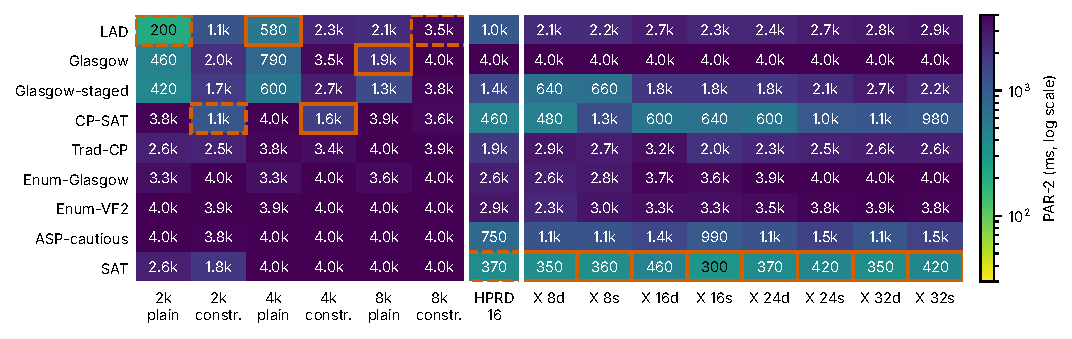
\includegraphics[width=\textwidth]{figures/fig3_strata.pdf}
\caption{Ancestor-equal PAR-2 (ms) per stratum: IdCon-Hard by host tier and variant, IdCon-HPRD, and IdCon-HPRD-X by query size and density. Boxes mark the best certified method per column (on Hard and HPRD, Glasgow-staged is a post hoc arm and is never boxed); a dashed box marks a column whose best and second-best methods are not distinguishable (bootstrap interval includes 0).}
\label{fig:strata}
\end{figure*}

\begin{table*}[t]
\caption{IdCon-Hard by stratum: ancestor-equal PAR-2 in ms (correct runs) and, last row, the bootstrap probability that the best certified method has the lowest PAR-2 with the 95\% interval of its difference to the runner-up (10,000 ancestor resamples, stratified by family; 12 ancestors per stratum, 2 per family). Best certified method in bold; $^{\circ}$the interval includes 0, so the best and second-best methods are not distinguishable. P(best) is the share of resamples in which the method is best, a stability measure rather than a probability of being best.}
\label{tab:strata-hard}
\centering\scriptsize\setlength{\tabcolsep}{2.5pt}
\begin{tabular}{lrrrrrr}
\toprule
Method & 2k plain & 4k plain & 8k plain & 2k constr. & 4k constr. & 8k constr.\\
\midrule
LAD & \textbf{196 (168)} & \textbf{580 (165)} & 2,108 (117) & 1,121 (147) & 2,306 (91) & \textbf{3,500 (37)}\\
Glasgow & 458 (154) & 789 (152) & \textbf{1,877 (120)} & 2,007 (104) & 3,548 (32) & 4,000 (0)\\
Glasgow-staged$^\dagger$ & 418 (154) & 602 (154) & 1,302 (138) & 1,693 (113) & 2,672 (73) & 3,751 (19)\\
CP-SAT & 3,842 (8) & 3,954 (2) & 3,925 (4) & \textbf{1,086 (142)} & \textbf{1,607 (137)} & 3,576 (28)\\
Trad-CP & 2,618 (76) & 3,758 (16) & 3,957 (2) & 2,481 (80) & 3,374 (33) & 3,895 (7)\\
Enum-Glasgow$^\ast$ & 3,319 (30) & 3,257 (34) & 3,550 (24) & 4,000 (0) & 4,000 (0) & 4,000 (0)\\
Enum-VF2$^\ast$ & 3,953 (2) & 3,866 (6) & 4,000 (0) & 3,887 (6) & 4,000 (0) & 4,000 (0)\\
ASP-cautious$^\ast$ & 3,963 (3) & 4,000 (0) & 4,000 (0) & 3,842 (12) & 4,000 (0) & 4,000 (0)\\
SAT$^\ddagger$ & 2,612 (95) & 3,953 (2) & 3,953 (2) & 1,844 (137) & 3,953 (2) & 3,953 (2)\\
First-match & 1,665 (100) & 2,391 (72) & 2,554 (76) & 1,032 (132) & 1,310 (133) & 2,455 (113)\\
\midrule
P(best) & LAD 0.75$^{\circ}$ & LAD 1.00 & Glasgow 0.99 & CP-SAT 0.63$^{\circ}$ & CP-SAT 1.00 & LAD 0.75$^{\circ}$\\
$\Delta$ to 2nd, 95\% CI & [-569, 44] & [-280, -139] & [-429, -32] & [-367, 299] & [-885, -512] & [-263, 110]\\
\bottomrule
\end{tabular}
\end{table*}

\begin{table*}[t]
\caption{IdCon-HPRD-X by stratum: ancestor-equal PAR-2 in ms (correct runs) and, last row, the bootstrap probability that the best certified method has the lowest PAR-2 with the 95\% interval of its difference to the runner-up (10,000 ancestor resamples). Best certified method in bold; $^{\circ}$the interval includes 0, so the best and second-best methods are not distinguishable. P(best) is the share of resamples in which the method is best, a stability measure rather than a probability of being best.}
\label{tab:strata-hprdx}
\centering\scriptsize\setlength{\tabcolsep}{2.5pt}
\begin{tabular}{lrrrrrrrr}
\toprule
Method & 8d & 8s & 16d & 16s & 24d & 24s & 32d & 32s\\
\midrule
LAD & 2,095 (32) & 2,165 (30) & 2,717 (21) & 2,310 (28) & 2,369 (27) & 2,695 (22) & 2,805 (21) & 2,948 (18)\\
Glasgow & 3,957 (1) & 4,000 (0) & 4,000 (0) & 4,000 (0) & 4,000 (0) & 4,000 (0) & 4,000 (0) & 4,000 (0)\\
Glasgow-staged & 644 (46) & 655 (46) & 1,812 (32) & 1,834 (32) & 1,845 (32) & 2,120 (28) & 2,714 (20) & 2,245 (29)\\
CP-SAT & 477 (48) & 1,257 (38) & 600 (48) & 638 (46) & 598 (48) & 1,025 (43) & 1,067 (44) & 978 (45)\\
Trad-CP & 2,858 (17) & 2,738 (21) & 3,200 (14) & 1,957 (34) & 2,265 (29) & 2,519 (26) & 2,645 (24) & 2,644 (26)\\
Enum-Glasgow$^\ast$ & 2,582 (26) & 2,816 (21) & 3,681 (7) & 3,556 (9) & 3,907 (2) & 4,000 (0) & 4,000 (0) & 4,000 (0)\\
Enum-VF2$^\ast$ & 2,267 (23) & 3,038 (14) & 3,304 (10) & 3,284 (10) & 3,451 (9) & 3,796 (3) & 3,903 (2) & 3,793 (3)\\
ASP-cautious$^\ast$ & 1,122 (46) & 1,112 (47) & 1,392 (45) & 986 (48) & 1,135 (47) & 1,531 (41) & 1,087 (48) & 1,476 (43)\\
SAT$^\ddagger$ & \textbf{354 (48)} & \textbf{359 (48)} & \textbf{461 (48)} & \textbf{299 (48)} & \textbf{374 (48)} & \textbf{423 (48)} & \textbf{351 (48)} & \textbf{420 (48)}\\
First-match & 2,363 (26) & 2,451 (24) & 2,205 (28) & 2,354 (26) & 2,275 (28) & 2,264 (28) & 1,773 (36) & 2,256 (28)\\
\midrule
P(best) & SAT 0.99 & SAT 1.00 & SAT 1.00 & SAT 1.00 & SAT 1.00 & SAT 1.00 & SAT 1.00 & SAT 1.00\\
$\Delta$ to 2nd, 95\% CI & [-250, -10] & [-630, -73] & [-221, -58] & [-696, -110] & [-306, -134] & [-1,179, -218] & [-1,268, -388] & [-1,044, -258]\\
\bottomrule
\end{tabular}
\end{table*}


\section{Further Tables}
Table~\ref{tab:repr} gives structural statistics, Table~\ref{tab:labels} correct runs by label, Table~\ref{tab:budget} completion at short budgets, Table~\ref{tab:scenario} IdCon-Hard by scenario, Table~\ref{tab:family} by graph family, and Table~\ref{tab:refs} the reference re-check and results restricted to fully confirmed references.
\begin{table}[t]
\caption{Structural statistics (medians over ancestors; for Hard the degree CV range over the six family medians in brackets). Candidate fraction: share of host entities that pass the degree filter and, where present, the unary domain of a non-anchored role.}
\label{tab:repr}
\centering\footnotesize
\setlength{\tabcolsep}{3pt}
\begin{tabular}{lrrrr}
\toprule
 & Hard plain & Hard constr. & HPRD & HPRD-X\\
\midrule
Host entities & 4,096 & 4,096 & 9,460 & 9,460\\
Mean degree & 4.0 & 4.0 & 7.4 & 7.4\\
Degree CV & 0.38 [0.00--1.54] & 0.38 [0.00--1.45] & 1.88 & 1.88\\
Clustering & 0.014 & 0.015 & 0.101 & 0.101\\
Pattern edges / role & 0.99 & 0.99 & 1.56 & 1.50\\
Candidate fraction & 0.919 & 0.925 & 0.113 & 0.097\\
\bottomrule
\end{tabular}
\end{table}

\begin{table}[t]
\caption{Correct runs by reference label, S/V/U/E for \Sat/\Vio/\Unk/\Emp{} (assessed runs per label in brackets). \Unk{} needs witnesses only; \Sat{}, \Vio{} and \Emp{} need an exhausted counterexample or existence search.}
\label{tab:labels}
\centering\footnotesize
\setlength{\tabcolsep}{2.4pt}
\begin{tabular}{lrrrr rrr}
\toprule
 & \multicolumn{4}{c}{IdCon-Hard} & \multicolumn{3}{c}{IdCon-HPRD-X}\\
\cmidrule(lr){2-5}\cmidrule(lr){6-8}
Method & S (342) & V (256) & U (322) & E (88) & S (38) & V (186) & U (160)\\
\midrule
LAD & 165 & 221 & 261 & 78 & 8 & 107 & 84\\
Glasgow & 104 & 169 & 237 & 52 & 0 & 1 & 0\\
Glasgow-staged$^\dagger$ & 125 & 197 & 262 & 67 & 14 & 136 & 115\\
CP-SAT & 145 & 80 & 37 & 59 & 38 & 177 & 145\\
Trad-CP & 59 & 49 & 68 & 38 & 19 & 90 & 82\\
Enum-Glasgow$^\ast$ & 24 & 12 & 26 & 26 & 1 & 28 & 36\\
Enum-VF2$^\ast$ & 0 & 0 & 6 & 8 & 5 & 15 & 54\\
ASP-cautious$^\ast$ & 6 & 3 & 6 & 0 & 38 & 176 & 151\\
SAT$^\ddagger$ & 99 & 62 & 45 & 34 & 38 & 186 & 160\\
\midrule
First-match & 306 & 235 & 6 & 79 & 38 & 186 & 0\\
\bottomrule
\end{tabular}
\end{table}

\begin{table}[t]
\caption{Correct runs within 0.5, 1 and 2\,s (read off the recorded end-to-end times of both repeats), and within 10\,s for repeat~0 (2\,s record if answered, otherwise the stage-2 rerun with a 10\,s budget; methods in that run only).}
\label{tab:budget}
\centering\footnotesize
\setlength{\tabcolsep}{1.9pt}
\begin{tabular}{lrrrr rrrr}
\toprule
 & \multicolumn{4}{c}{IdCon-Hard} & \multicolumn{4}{c}{IdCon-HPRD}\\
\cmidrule(lr){2-5}\cmidrule(lr){6-9}
Method & 0.5\,s & 1\,s & 2\,s & 10\,s$^{0}$ & 0.5\,s & 1\,s & 2\,s & 10\,s$^{0}$\\
\midrule
LAD & 360 & 526 & 725 & 460/504 & 0 & 281 & 389 & 200/200\\
Glasgow & 314 & 421 & 562 & -- & 0 & 0 & 0 & 184/200\\
Glasgow-staged$^\dagger$ & 403 & 539 & 651 & 400/504 & 243 & 271 & 304 & 194/200\\
CP-SAT & 97 & 213 & 321 & 231/504 & 377 & 384 & 384 & 196/200\\
Trad-CP & 55 & 126 & 214 & -- & 49 & 188 & 279 & --\\
Enum-Glasgow$^\ast$ & 64 & 75 & 88 & 44/504 & 0 & 0 & 235 & 198/200\\
Enum-VF2$^\ast$ & 8 & 12 & 14 & -- & 56 & 98 & 127 & --\\
ASP-cautious$^\ast$ & 0 & 0 & 15 & -- & 47 & 361 & 400 & --\\
SAT$^\ddagger$ & 16 & 24 & 240 & -- & 315 & 400 & 400 & --\\
\midrule
First-match & 327 & 498 & 626 & -- & 38 & 230 & 230 & --\\
\bottomrule
\end{tabular}
\end{table}

\begin{table}[t]
\caption{IdCon-Hard by scenario: assessed references (\Sat/\Vio/\Unk/\Emp) and first-match errors among assessed runs. \textsf{decoy\_s} is a predicate-range control (Amendment~1).}
\label{tab:scenario}
\centering\footnotesize
\begin{tabular}{lrr}
\toprule
Scenario & Labels & First-match wrong\\
\midrule
\textsf{decoy\_v} & 44/0/28/0 & 56/144\\
\textsf{decoy\_u} & 43/0/29/0 & 54/144\\
\textsf{decoy\_s} & 0/72/0/0 & 0/144\\
\textsf{focal\_v} & 0/56/16/0 & 32/144\\
\textsf{mixed} & 34/0/38/0 & 73/144\\
\textsf{background} & 42/0/30/0 & 60/144\\
\textsf{perturbed} & 8/0/20/44 & 40/144\\
\bottomrule
\end{tabular}
\end{table}

\begin{table}[t]
\caption{IdCon-Hard ancestor-equal PAR-2 (ms) by graph family (12 ancestors each). Best certified method per family in bold.}
\label{tab:family}
\centering\footnotesize
\setlength{\tabcolsep}{3pt}
\begin{tabular}{lrrrrrr}
\toprule
Method & Artic. & ER & Geom. & PA & Reg. & SW\\
\midrule
LAD & \textbf{1,303} & \textbf{1,535} & \textbf{2,484} & \textbf{1,404} & \textbf{1,500} & \textbf{1,584}\\
Glasgow & 1,797 & 2,141 & 3,088 & 1,873 & 1,767 & 2,012\\
Glasgow-staged$^\dagger$ & 1,273 & 1,887 & 2,832 & 1,460 & 1,399 & 1,586\\
CP-SAT & 2,661 & 2,776 & 3,813 & 2,938 & 2,852 & 2,950\\
Trad-CP & 2,649 & 3,537 & 4,000 & 2,376 & 3,633 & 3,888\\
Enum-Glasgow$^\ast$ & 3,953 & 3,875 & 3,459 & 3,648 & 3,721 & 3,469\\
Enum-VF2$^\ast$ & 4,000 & 3,960 & 4,000 & 3,907 & 3,838 & 4,000\\
ASP-cautious$^\ast$ & 3,806 & 4,000 & 4,000 & 4,000 & 4,000 & 4,000\\
SAT$^\ddagger$ & 3,154 & 3,258 & 4,000 & 3,338 & 3,268 & 3,251\\
\midrule
First-match & 2,077 & 1,423 & 2,628 & 2,243 & 1,846 & 1,189\\
\bottomrule
\end{tabular}
\end{table}

\begin{table}[t]
\caption{Reference quality. Non-trivial negative states (not excluded by the observation tables) and how many a second engine confirms, after stage~1 and after the stage-2 re-check; ancestor-equal PAR-2 (ms) on all assessed references and on references whose every non-trivial negative is confirmed.}
\label{tab:refs}
\centering\footnotesize
\setlength{\tabcolsep}{3pt}
\begin{tabular}{lrrrrrr}
\toprule
 & \multicolumn{2}{c}{Hard} & \multicolumn{2}{c}{HPRD} & \multicolumn{2}{c}{HPRD-X}\\
\cmidrule(lr){2-3}\cmidrule(lr){4-5}\cmidrule(lr){6-7}
 & all & confirmed & all & confirmed & all & confirmed\\
\midrule
Negatives, stage 1 & 301 & 187 & 115 & 115 & -- & --\\
Negatives, stage 2 & 305 & 285 & 115 & 115 & 112 & 111\\
Tasks & 504 & 487 & 200 & 200 & 192 & 191\\
\midrule
LAD & 1,635 & 1,618 & 1,036 & 1,036 & 2,513 & 2,498\\
Glasgow & 2,113 & 2,072 & 4,000 & 4,000 & 3,995 & 3,995\\
Glasgow-staged$^\dagger$ & 1,740 & 1,694 & 1,361 & 1,361 & 1,734 & 1,734\\
CP-SAT & 2,998 & 3,003 & 455 & 455 & 830 & 829\\
Trad-CP & 3,347 & 3,354 & 1,858 & 1,858 & 2,603 & 2,603\\
Enum-Glasgow$^\ast$ & 3,688 & 3,690 & 2,638 & 2,638 & 3,568 & 3,568\\
Enum-VF2$^\ast$ & 3,951 & 3,951 & 2,937 & 2,937 & 3,354 & 3,354\\
ASP-cautious$^\ast$ & 3,968 & 3,968 & 748 & 748 & 1,230 & 1,227\\
SAT$^\ddagger$ & 3,378 & 3,386 & 374 & 374 & 380 & 380\\
First-match & 1,901 & 1,916 & 2,027 & 2,027 & 2,242 & 2,241\\
\bottomrule
\end{tabular}
\end{table}


\section{Reproduction Checklist}
Verify record hashes; install the pinned Python dependencies (\path{requirements.txt}); build the patched LAD2025 binary, Glasgow at commit \texttt{01ef6ca}, CaDiCaL 2.1.3 and drat-trim; run \texttt{tools/verify.py}, which recomputes every table and macro of this paper from the frozen records without timing anything; fetch the upstream HPRD, CEMR and Planetoid files, regenerate the inputs and check their hashes; rerun the independent check with \path{experiment/independent/idcheck.py}. New timing runs should use a new output directory and be reported as new results.

\clearpage
\end{document}
